\documentclass[11pt]{article}
\usepackage[utf8]{inputenc}
\usepackage[a4paper, margin=1in]{geometry}
\usepackage{amsmath}
\usepackage[spanish]{babel}
\usepackage{graphicx}
\usepackage{subcaption}
\usepackage{pdfpages}
\usepackage{wrapfig}
\usepackage[separate-uncertainty=true, locale=FR]{siunitx}
\usepackage{hyperref}
\usepackage{tcolorbox}
\newcommand{\polar}[0]{PolaRx5\textsuperscript{TR}}
\newcommand{\BNC}[0]{Berkeley Nucleonics 1105}

%% biblatex
\usepackage[style = numeric, backend = biber, sorting = none, doi = false, isbn = false, url = true]{biblatex}
% \usepackage[defernumbers = true, style = numeric, backend = biber, sorting = none, doi = false, isbn = false, url = true]{biblatex}
% \usepackage[style = numeric, backend = biber, sorting = none]{biblatex}    % REFERENCIAS como section
\AtEveryBibitem{
    \clearfield{urlyear}
    \clearfield{urlmonth}
} % Do not show the "(visited on <date>)" on the references
\DefineBibliographyStrings{spanish}{}
\usepackage{csquotes}
\addbibresource{./calValGNSS.bib}
\renewcommand*{\bibfont}{\fontsize{9}{12}\selectfont}


\title{Cuaderno de laboratorio, receptor viajero} 
\author{Victor Bettachini, Diego Luna}
\date{2024}

\begin{document}

\maketitle


%\begin{abstract}
%Este documento describe un proyecto para la generación de una red de comparación de relojes atómicos de la Argentina. La red funcionará como una herramienta para la evaluación de las referencias de tiempo y frecuencia utilizadas en laboratorios de investigación. Se espera que este proyecto sirva no sólo a fines académicos, sino que acompañe el desarrollo de actividades dependientes de referencias exactas de tiempo y frecuencia, como las telecomunicaciones, la metrología o el sincronismo en redes. 
%\end{abstract}


\newpage
\tableofcontents
\newpage





\section{08/02/2024. Primeras mediciones de delays}

El cable de antena tiene terminales TNC macho.
Se utilizaron adaptadores TNC hembra a BNC macho para conectarle con el instrumento y otros cables.



\subsection{Tx con T de BNC}

La primer medición intentada fue una variante propia de la técnica de transmisión, ``1PSS Tx'', donde una única señal del distribuidor de PPS se dividió en una T de BNC.
La PPS se alimentó a un brazo de una T de BNC conectada en el canal 1 del TIC.
Al otro brazo se conectó un cable, cuyo restraso se mide como tara, que finalizó en el canal 2.
Registrado el intervalo $1 - 2$ se obtuvo el retraso en ese cable, \SI{50.2}{\nano\second}.
Tal medición fue simple, no es el promedio de varias y lo expresado en pantalla tiene 1 dígito para la décima de \si{\nano\second}.

Con un tambor BNC hembra-hembra se intercaló el cable de antena entre la T de BNC y el canal 2.
El orden fue brazo de T de BNC, adaptador TNC-BNC, cable de antena, adaptador TNC-BNC, cable adicional, tambor, terminal BNC hmebra del canal 2 del TIC.
Esta configuración la ilustra la figura \ref{fig:TXtrucho}.

\begin{figure}[ht]
    \begin{center}
        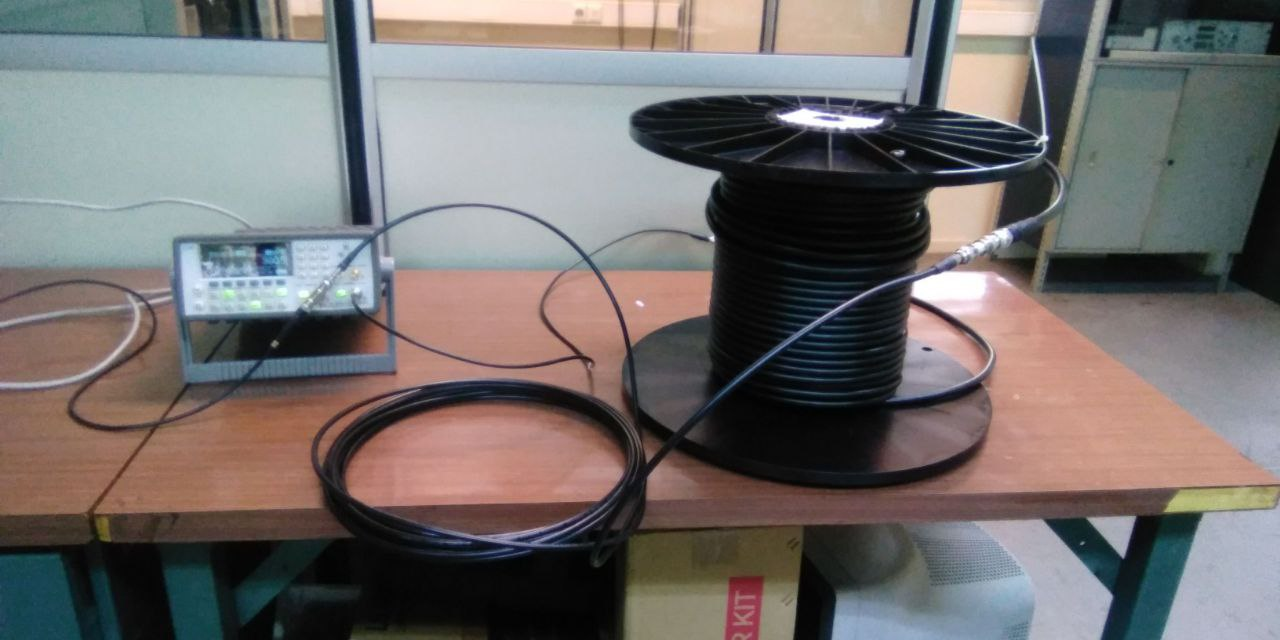
\includegraphics[width=0.8\textwidth]{./figuras/2.jpg}
        \caption{Delay cable antena}
        \label{fig:TXtrucho}
    \end{center}
\end{figure}

En esta configuración la medición arrojó el resultado \SI{380.9}{\nano\second}.
Decontando la diferencia de la medición solo con el cable auxiliar el retraso en el cable de antena medido fue de \SI{328.9\pm0.2}{\nano\second}.


\subsection{Tx con dos PPS}

En la bibliografía de referencia  \cite{rovera_techniques_2015} la sugerencia para implementar la técnica de medición por transmisión es la de utilizar dos señales del distribuidor de PPS y dividir una única, como se hizo con la T de BNC.
Para implementar esta medición por transmisión ``1PPS Tx'' dos cable con terminales BNC conectan dos distintos terminales del distribuidor de PPS a sendos canales del TIC.
Con una impedancia de entrada de \SI{50}{\ohm}, acoplamiento de corriente continua (DC) y un nivel de disparo (trigger) de \SI{0.5}{\volt} la diferencia entre el canal 2 y el canal 1 fue de \SI{20.8\pm0.1}{\nano\second}.

Para medir el retraso intercalando el cable de antena se procedió de igual forma que en la medición anterior, a utilizar un tambor BNC con terminales hembra para conectar el cable que iba del distribuidor al canal 2 con el de antena y este se conecte a la entrada del canal 2 del TIC.
En esta condición se registró un retraso entre canales de \SI{349.5\pm0.1}{\nano\second}, con lo que el retraso de señal en la antena medido es de \SI{328.7\pm0.2}{\nano\second}.

Para cuantificar la dispersión de las mediciones una serie de 100 muestras mostró un desvío estándar en la muestra de \SI{0.06}{\nano\second}.




\subsection{Rx con T de BNC}\label{sec:Rx}

La técnica utiliza dos señales 1PPS tomadas desde el distribuidor.
Uno de los cables con esta señal se conecta a la entrada del canal 1 de medición del TIC.
Este se ajusta para tener un umbral (threshold) de \SI{0.5}{\volt}, acoplamiento de corriente continua (DC) y una impedancia de entrada de \SI{50}{\ohm}.
En el canal 2 del TIC se conecta el pie de una T de BNC.
En uno de sus brazos conecta a un cable que trae la segunda señal 1PPS del distribuidor.
El brazo restante se utiliza como terminal de medición.
A diferencia de lo ajusta para el canal 1, el canal 2 del TIC deberá presentar una alta impedancia de entrada, \SI{1}{\mega\ohm}, y una nivel de umbral alto, \SI{5}{\volt}, pero mantiene el acoplamiento de corriente continua (DC).
El objeto de estos ajustes es que sea sensible al rebote de las señal que producirá en el extremo que se deje libre.

La medición de tara se realiza dejando libre el brazo de la T de BNC.
Puesto que registra primero la señal ascendente en el otro canal, la tara es la diferencia con \SI{1}{\second} de lo mostrado en pantalla.
Para una serie de 100 mediciones esto fue \SI{0.99999998278}{\second}, con un desvío estándar de \SI{1.2}{\nano\second} por lo que la tara es \SI{17.2\pm1.2}{\nano\second}.

La medición del retraso en el cable de la antena se efectua conectando un terminal de la misma al brazo que estaba libre de la T de BNC.
El otro extremo del cable de antena debe quedar libre, con lo que la configución para esta metodología de medición es la que la que muestra la figura \ref{fig:RxRovera}.

\begin{figure}[ht]
    \begin{center}
        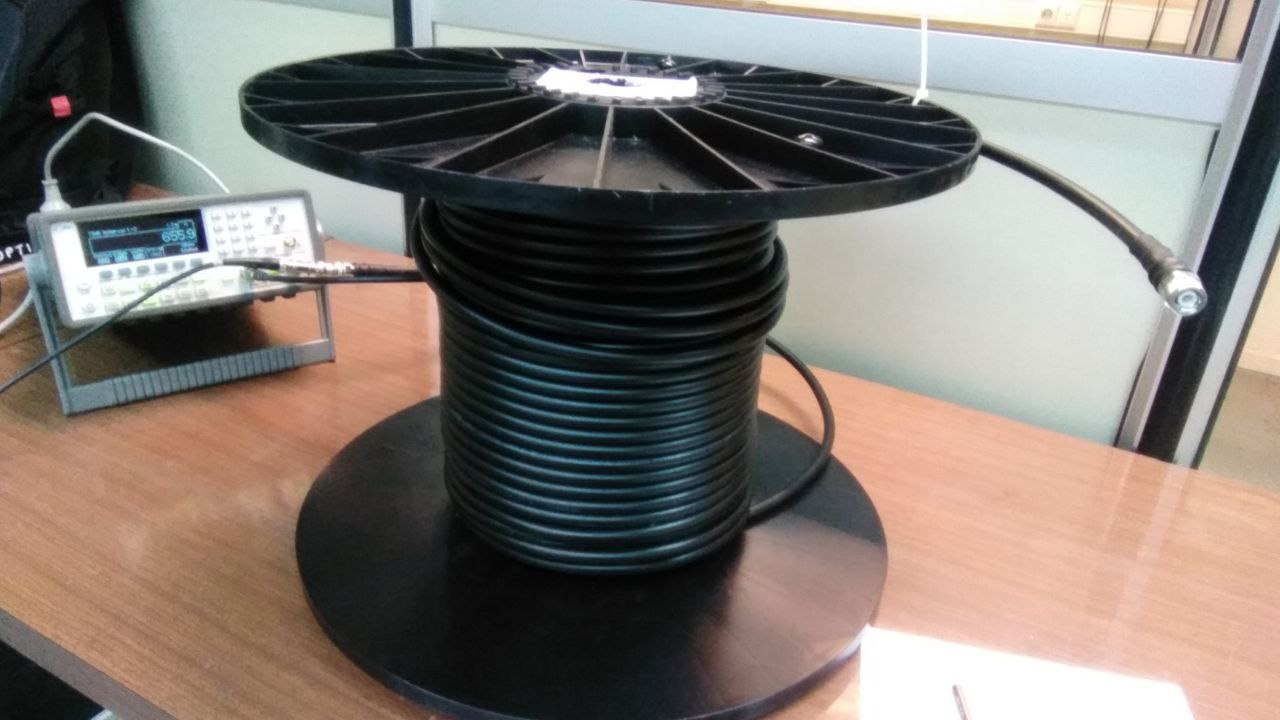
\includegraphics[width=0.8\textwidth]{./figuras/4.jpg}
        \caption{Delay cable antena}
        \label{fig:RxRovera}
    \end{center}
\end{figure}

Una medición promediando 100 registros mostró en pantalla un diferencia entre los canales de \SI{635.91}{\nano\second} con un desvío estándar de la muestra de \SI{0.08}{\nano\second}.
Este resultó ser ligeramente superior que la medición de transmisión, lo que concuerda con la afirmación expresada en \cite{rovera_techniques_2015} de que la técnica de transmisión (TX) es más precisa (mayor estabilidad) que la realizada por reflexión (RX).

\section{09/02/2024. Medición delay de antena viajera}

Se repite la medición del 8 de febrero para el delay de la antena. El rollo de cable se mantuvo dentro del recinto de relojes para su estabilización térmica. Según los registros del sensor, la temperatura fue de \SI{18}{\celsius}. Luego se retiró el rollo y se midió inmediatamente según el esquema de la figura \ref{fig:cabledelay}. 


\begin{figure}[ht]
    \begin{center}
        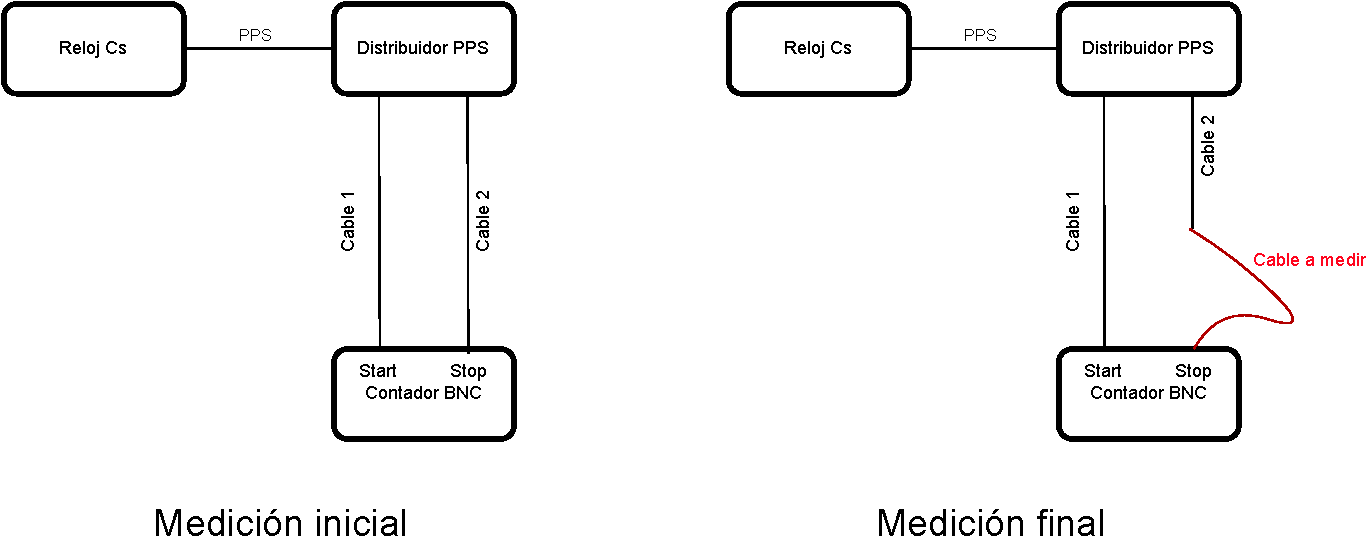
\includegraphics[width=1\textwidth]{./figuras/cabledelay}
        \caption{Esquema de medición}
        \label{fig:cabledelay}
    \end{center}
\end{figure}

El resultado coincide con el de ayer. Por lo tanto, tomamos como valor de delay del cable de antena:


\begin{equation}
\boxed{X_C=\SI{328,7(0,06)}{\nano\second}}\label{eq:Xc} 
\end{equation}

Se utilizó un valor de trigger de \SI{1}{\volt}. La incertidumbre asignada en la ecuación \ref{eq:Xc} corresponde al desvío estándar de 100 mediciones ($k=1$). Notar que para esta medición se usaron adaptadores TNC-hembra a BNC-macho en los extremos del cable, junto con un conector BNC hembra-hembra.
El modelo del cable es LMR-LW400 Times Microwave Systems, con fecha de fabricado en mayo del 2021.



Se identificaron los cables viajeros como ``A'' y ``B''. A modo de referencia, el delay del cable ``A'' es de \SI{46,5(0,08)}{\nano\second} y el del cable ``B'' es de \SI{61,9(0,08)}{\nano\second}.


\section{14/02/2024. Montaje antena, medición de Rise time y delay de cable}

\subsection{Montaje antena}

Se montó la antena en la terraza de INTI. Se muestran las fotos en \ref{fig:antenaINTI}. Según el GPS del celular, la altura es de \SI{37.8} MSNM.


\begin{figure}[ht]
    \begin{center}
        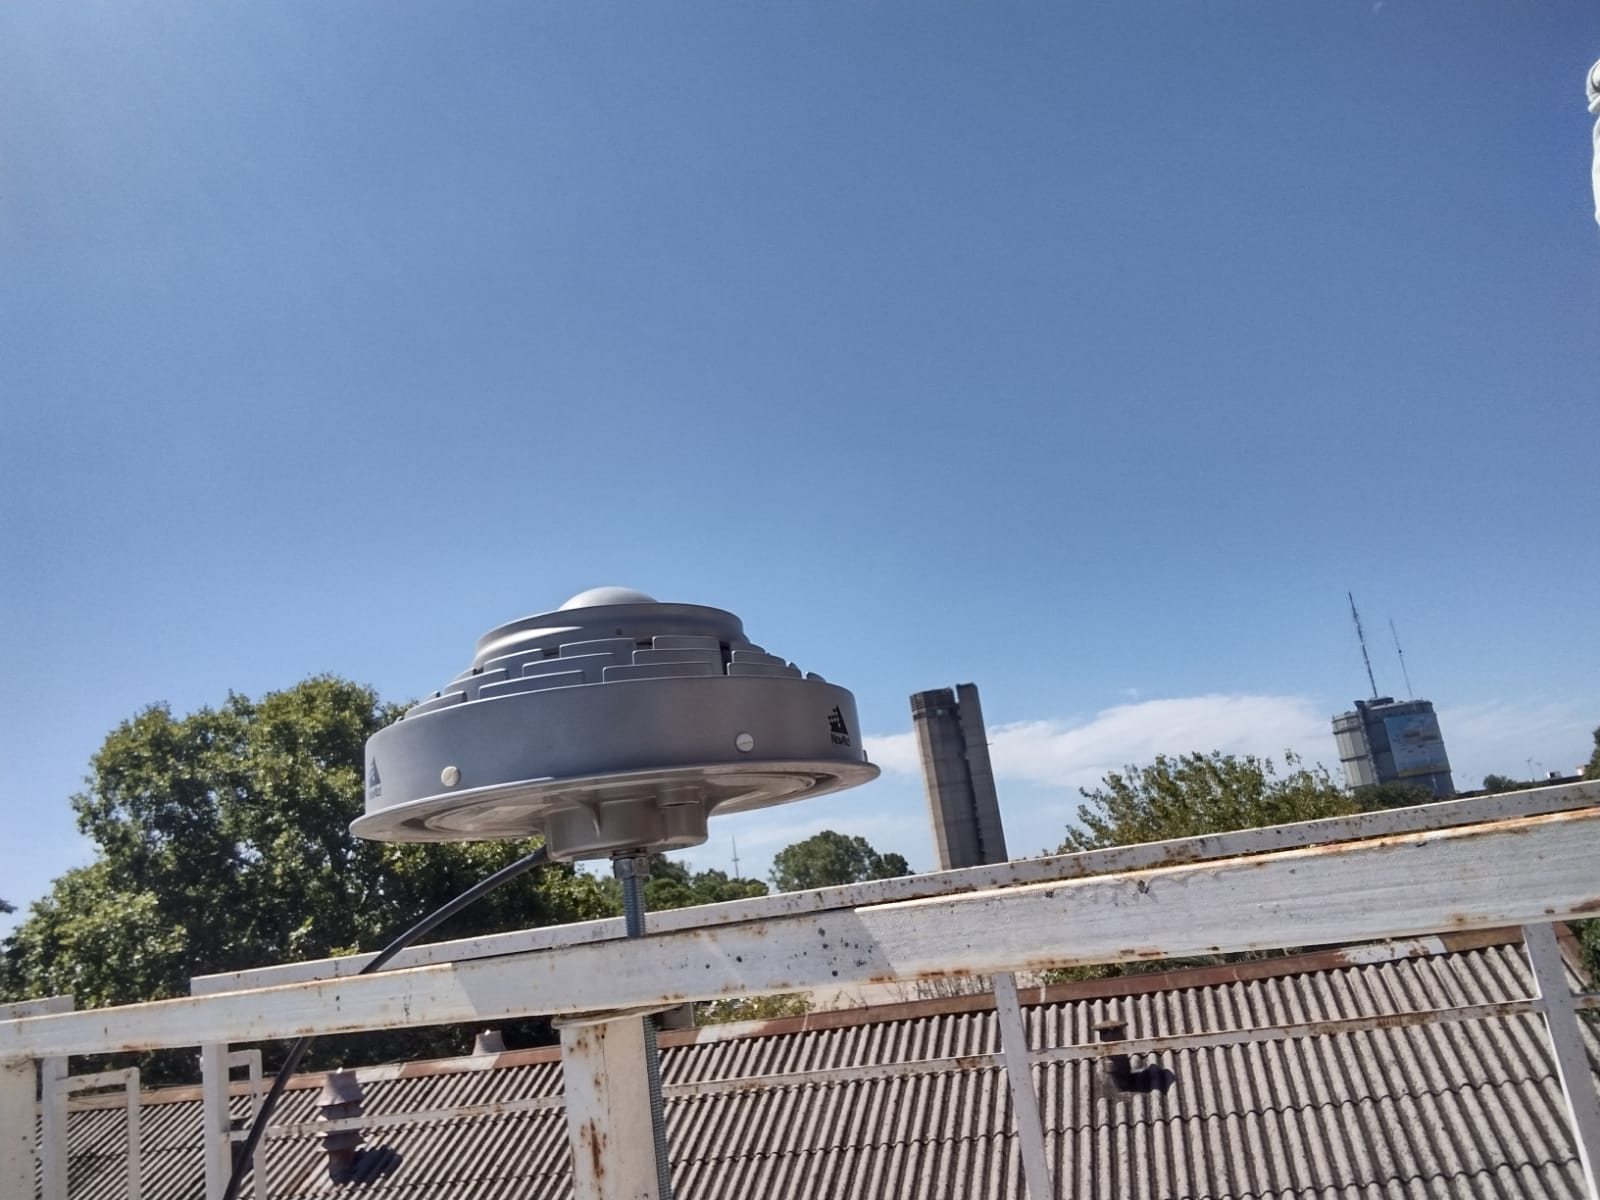
\includegraphics[width=0.4\textwidth]{./figuras/AntenaSIM1}
            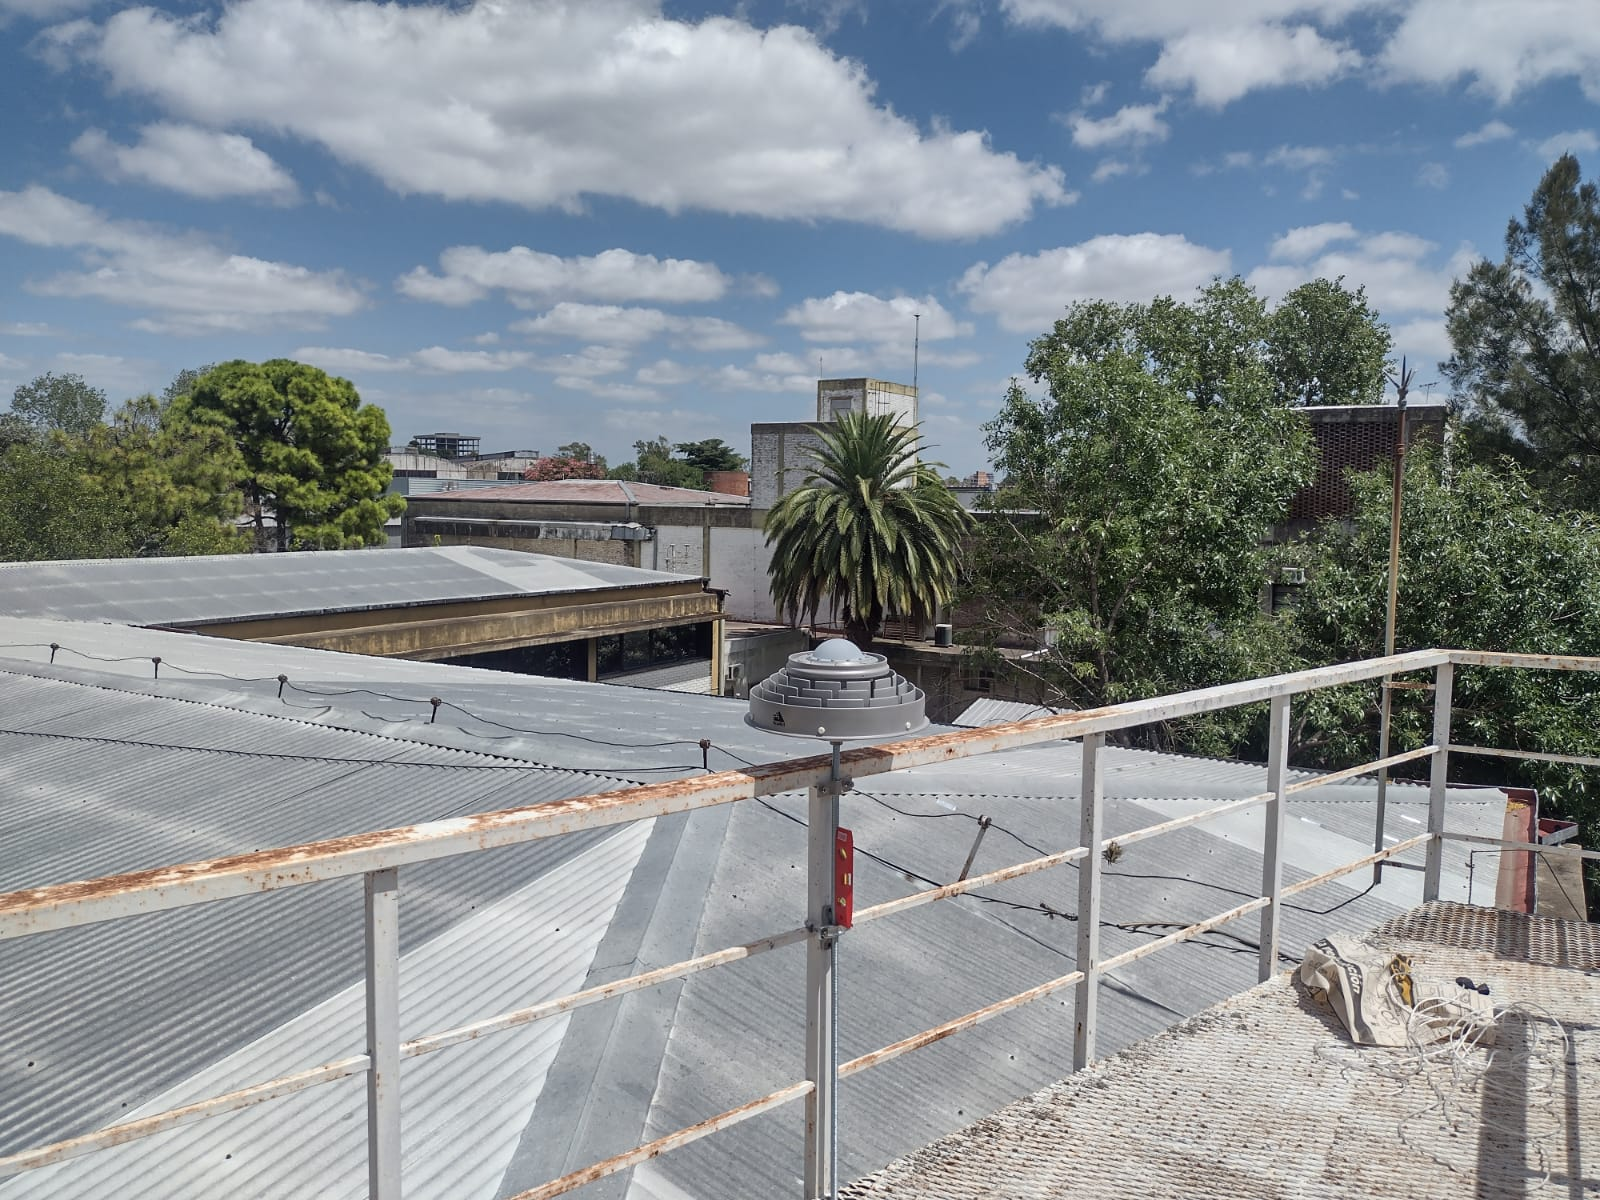
\includegraphics[width=0.4\textwidth]{./figuras/AntenaSIM2}
            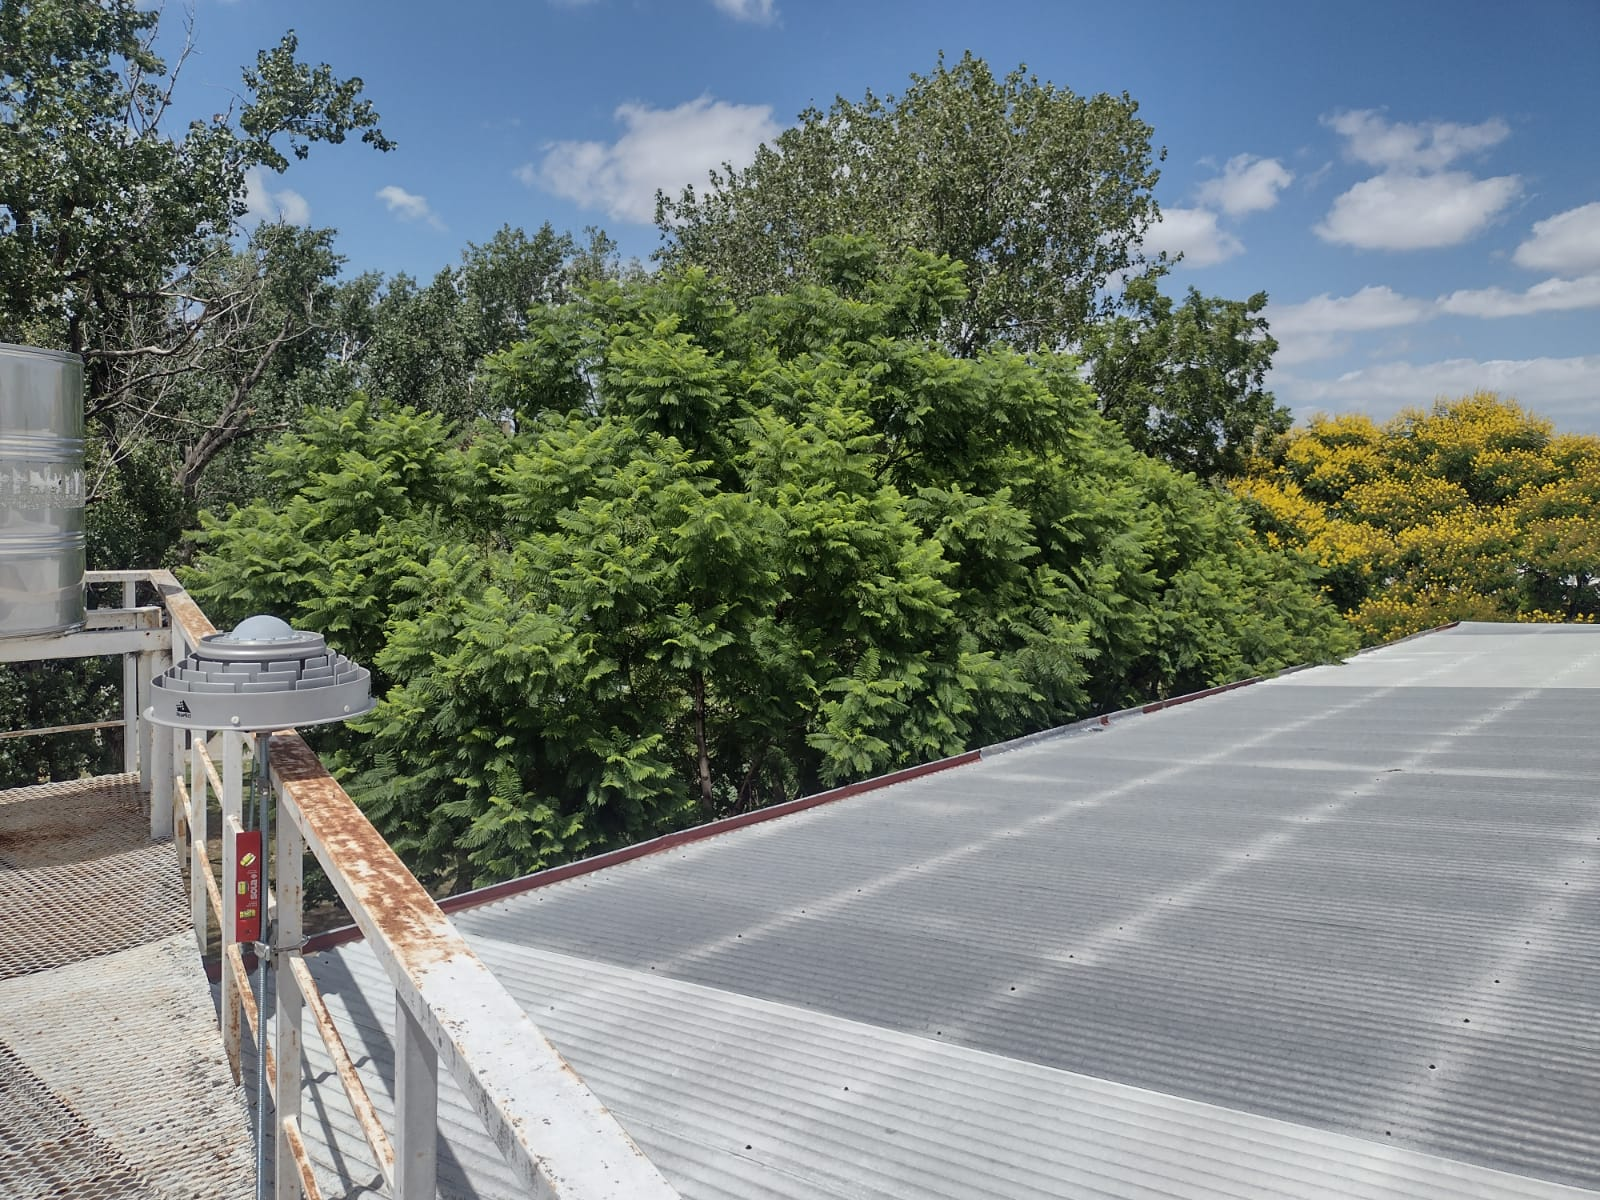
\includegraphics[width=0.4\textwidth]{./figuras/AntenaSIM3}
            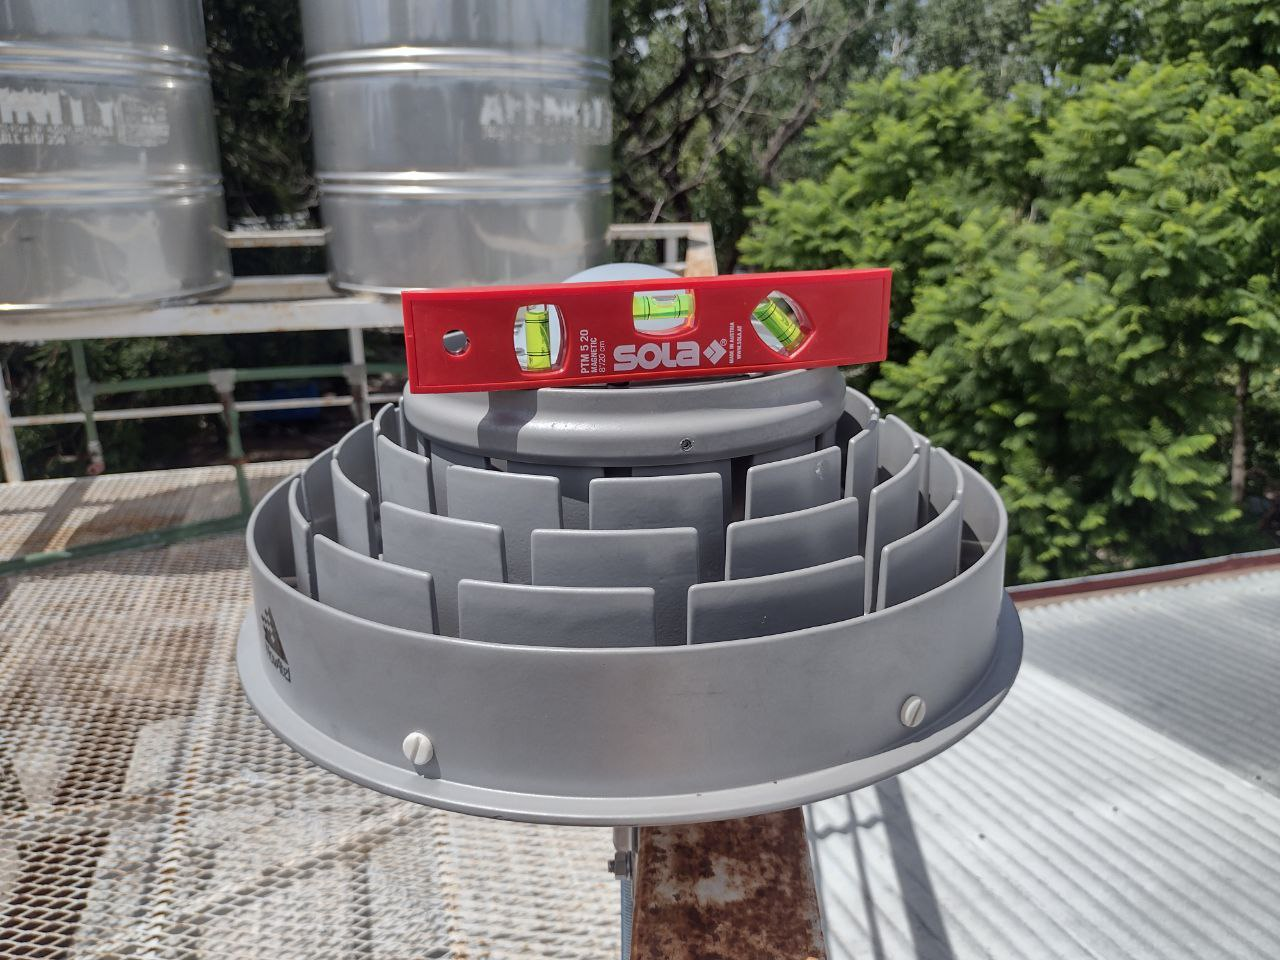
\includegraphics[width=0.4\textwidth]{./figuras/AntenaSIM4}
        \caption{Montaje antena en INTI}
        \label{fig:antenaINTI}
    \end{center}
\end{figure}


\subsection{Rise time}
Intento medir el Rise time con el contador BNC. No lo logro. intento con el contador Agilent del laboratorio, pero tampoco. Según la especificación del distribuidor de pulsos, Microsemi 4033A, el Rise time debería se menor a \SI{2}{\nano\second}. Lo que puede suceder es que el pulso esté por fuera del rango de medición de los contadores. De todas maneras, pruebo con el generador digital UNI-T y genero un valor de Rise time de \SI{10}{\micro\second}. Tampoco logro medirlo con el contador BNC. No lo intenté con el Agilent.

\begin{figure}[ht]
    \begin{center}
        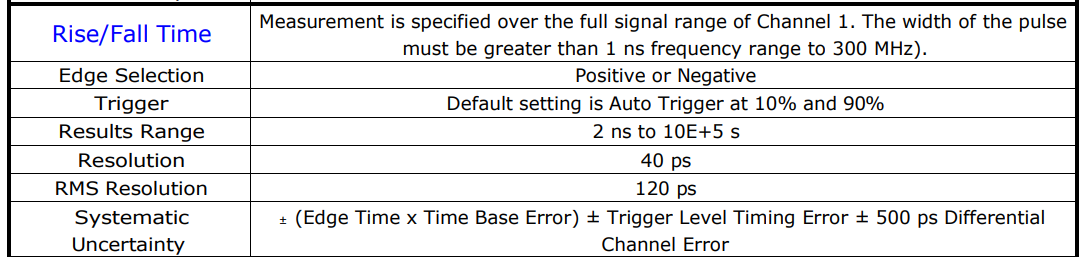
\includegraphics[width=0.7\textwidth]{./figuras/RiseTimeSpecsBNC}
        \caption{Rise Time specs del BNC counter}
%        \label{fig:Rise Time specs del BNC counter}
    \end{center}
\end{figure}

\subsection{Delay cable receptor}
Se etiquetó un cable como \textbf{PPS SIM Receiver}. El delay medido resultó:


\begin{equation}
\boxed{X_{P}=\SI{5.5(0,06)}{\nano\second}}%\label{eq:X0} 
\end{equation}

Para alimentar el receptor viajero, lo conecto a la salida 9 del distribuidor de pulsos.

\section{15/02/2024. Medición de delay de cable montado}

Con el cable de la antena montado, le vuelvo a medir el delay. Uso el método \textit{Rx con T} de la sección  \ref{sec:Rx}. Uso el contador Agilent con promedio de 100 mediciones.

\begin{table}[ht]
    \centering
    \begin{tabular}{|c||c|}
        \hline
        Hora & Resultado (Agilent counter)\\
        \hline
        10:30 & \SI{337.3}{\nano\second} \\
        11:00 & \SI{337.4}{\nano\second}\\
        12:00 & \SI{337.4}{\nano\second}\\
        13:30 & \SI{337.4}{\nano\second}\\
        15:30 & \SI{337.6}{\nano\second}\\
        \hline
    \end{tabular}
    \caption{Mediciones de delay de cable de antena montado, para el 2024-02-15. El resultado del 13/2 fue \SI{328.7}{\nano\second} con el contador BNC. }
    \label{tab:my_label}
\end{table}

Durante el día, el valor se mantiene estable dentro de la décima de ns. Sin embargo, no coincide con la medición del 13/2. Repito por si se trata de una cuestión del contador. Ahora uso el BNC counter tabla \ref{tab:delayconBNC}).

\begin{table}[ht]
    \centering
    \begin{tabular}{|c||c|}
        \hline
        Hora & Resultado (BNC counter)\\
        \hline
        14:00 & \SI{336.9}{\nano\second} \\
        15:30 & \SI{336.7}{\nano\second} \\
        \hline
    \end{tabular}
    \caption{Mediciones de delay de cable de antena montado, para el 2024-02-15. El resultado del 13/2 fue \SI{328.7}{\nano\second} con el contador BNC.  }
    \label{tab:delayconBNC}
\end{table}

Ahora con el SR620, con la misma medicion (tabla \ref{tab:delayconSR620})


\begin{table}[ht]
    \centering
    \begin{tabular}{|c||c|}
        \hline
        Hora & Resultado (SR620 counter)\\
        \hline
        14:30 & \SI{341.7}{\nano\second} \\
        \hline
    \end{tabular}
    \caption{Mediciones de delay de cable de antena montado, para el 2024-02-15. El resultado del 13/2 fue \SI{328.7}{\nano\second} con el contador SR620.  }
    \label{tab:delayconSR620}
\end{table}


\section{16/02/2024. Medición de variación de delay en cable antena durante un día}

Voy a hacer mediciones durante todo el tiempo que esté en INTI, cada una hora (tabla \ref{tab:delayTodoUnDia}). Noto algo muy raro: Si se usa el contador BNC con base de tiempo externa, la lectura de delay es incorrecta (!!!!). Entre conectar y desconectar los 10 MHz del cesio, la lectura pasa de unos 640 a 290 ns. Hay que investigar esto.


\begin{table}[ht]
    \centering
    \begin{tabular}{|c||c|c|}
        \hline
        Hora(Arg.) & Contador BNC  & Contador Agilent\\
        \hline
        11:00 & \SI{336.66}{\nano\second} & \SI{337.55}{\nano\second}  \\
        12:00 & \SI{336.61}{\nano\second} & \SI{337.57}{\nano\second}  \\
        13:00 & \SI{336.62}{\nano\second} & \SI{337.58}{\nano\second}  \\
        14:00 & \SI{336.67}{\nano\second} & \SI{337.58}{\nano\second}  \\
        15:00 & \SI{336.66}{\nano\second} & \SI{337.57}{\nano\second}  \\
        16:00 & \SI{336.61}{\nano\second} & \SI{337.59}{\nano\second}  \\

        \hline
    \end{tabular}
        \caption{Mediciones de delay de cable de antena montado, para el 2024-02-16. }
    \label{tab:delayTodoUnDia}
\end{table}

\section{19/02/2024. Comienzo de mediciones}
Largamos las mediciones con Víctor. Medimos el $X_0$ del receptor \polar. Nos da $\SI{96.7}{\nano\second}-\SI{41.5}{\nano\second}=\SI{55.2}{\nano\second}$

\begin{equation}
\boxed{X_0=\SI{55.2}{\nano\second}}\label{eq:X0} 
\end{equation}

Teniendo en cuenta el delay del cable del día 14/2/2024, el valor de REFDLY da:

\begin{equation}
\boxed{REFDLY_{\polar}=\SI{60.7}{\nano\second}}\label{eq:REFDLY} 
\end{equation}



\section{20/02/2024.}
Los CGGTTS siguen arrojando mediciones erróneas. Veo que la antena (Novatel GNSS-750) trabaja con tensiones entre 3.3 y 12 V. El receptor entrega 5 V nominales. Lo mido a la salida del receptor y me da 4.96 V. Al final del cable, da igual, 4.96 V (!).


Por recomendación de Bijunath, mido la potencia de la señal de 10 MHz de entrada al receptor, figura \ref{fig:espectro10MHz}. Me da alrededor de 7 dBm. Está bien porque en el manual del receptor \polar dice que admite entre  -8 dBm y + 18 dBm.

\begin{figure}[ht]
    \begin{center}
        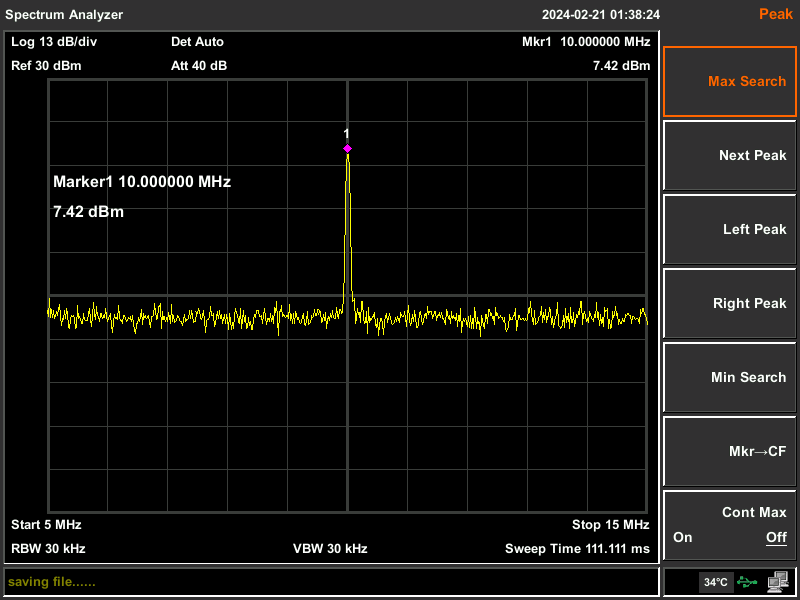
\includegraphics[width=0.4\textwidth]{./figuras/espectro10MHz}
        \caption{Espectro de los 10 MHz a la salida del distribuidor, entrada del \polar}
        \label{fig:espectro10MHz}
    \end{center}
\end{figure}

Escribo a Bijunath y le cuento que me da un poco menos de 50 dB en los tres satélites. (ver correos del dia de hoy). También me parece un poco pequeña la altura de la señal en el espectro L2 (\SI{1227,6}{\mega\hertz} )


\section{21/02/2024. Hago pruebas sugeridas por Bijunath.}

Estas son las sugerencias de Bijunath:

I can say the receiver was tested and operated for slightly more than two weeks before it was shipped out.

Regardless, it’s still under warranty from Septentrio. It’s brand new.

Here are the things I’d try:

Run the receiver in disciplined mode and compare the PPs-out with your local clock.
                 You should be able to see +/- 20 ns.

If 1) doesn’t work, it could be that the antenna or the receiver is broken.
If 1) looks good, refer to the Timing Mode settings and check whether the System time is set to external clk when the receiver is operating with external clk input. Compensated or uncompensated mode doesn’t provide you with any useful information; the difference is typically ~0.5 ns
Then, check whether the PPS is synced. with the 10 MHz clock.
Send me the Rx control picture while the receiver is in operation for both steered and clk input modes that have the clk bias information. Also, remind me of the S/N. I don’t remember that.
 

If everything thing you try fails, you may have to contact Septentrio support. All they need is the S/N.\\

RESPUESTAS:\\

Me dí cuenta de que los 10 MHz de salida no estaban habilitados en la interfaz del \polar. Cuando lo activo, genera la señal de 10 MHz, casi coincidente con todas las cifras del contador.

Mido el PPS generado a partir de GPS. Comparando con la red del SIM, la diferencia es de \SI{10}{\nano\second}, aproximadamente. No hay problema con eso. 
Sin embargo, los CGGTTS se siguen generando mal (valores sin sentido). 

Intento largar una medición desde el software dedicado que vino instalado en la notebook, pero sólo logro generar RINEX.


\section{22/02/2024. Comienzo medición larga GNSS}

Comienzo medición con el \polar. Lo configuro según la figura \ref{fig:22feb24}. Como  $X_0$ inicial tomo el del 19/2. Cuando termine la medición GPS, lo vamos a volver a medir.



\begin{figure}[ht]
    \begin{center}
        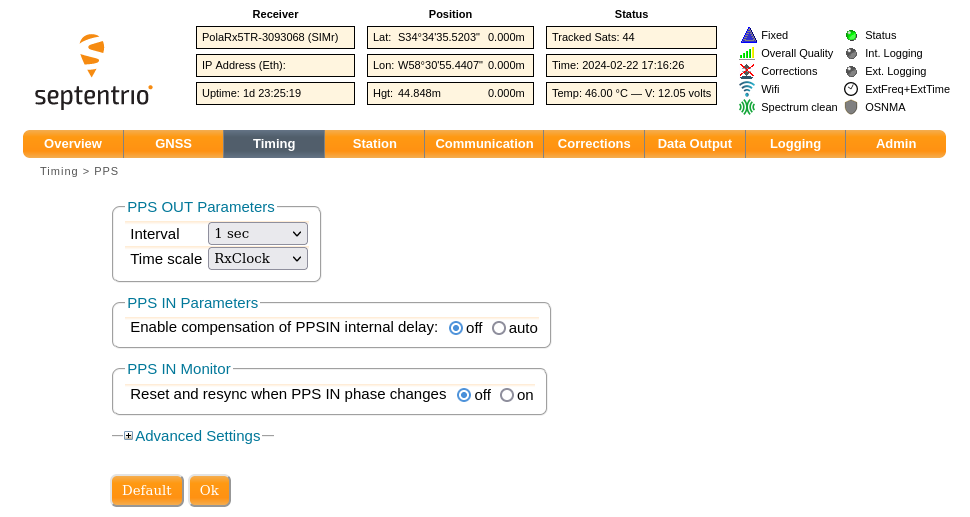
\includegraphics[width=0.4\textwidth]{./figuras/Screenshot from 2024-02-22 17-20-29.png}
        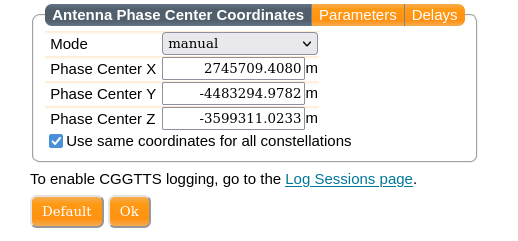
\includegraphics[width=0.4\textwidth]{./figuras/Screenshot from 2024-02-22 17-21-05.png}
        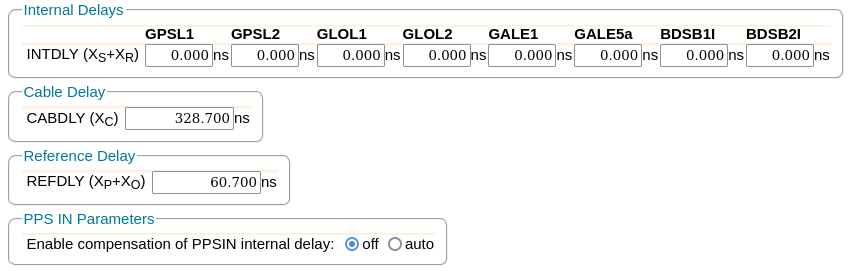
\includegraphics[width=0.6\textwidth]{./figuras/Screenshot from 2024-02-22 17-21-41.png}
        \caption{Configuración de receptor \polar.}
        \label{fig:22feb24}
    \end{center}
\end{figure}

\section{22/02/2024. Medición de Rise Time con el \BNC}
Pruebo medir Rise Time con el BNC y el generador de funciones UNI-T. Funciona bien hasta el mínimo que puede generar el contador: \SI{15}{\nano\second}. La configuración del BNC es: Trigger:AUTO, Sens:MIDDLE, Imp:\SI{1}{\mega\ohm}, Couple:AC.

Intento usar esa configuración para medir los pulsos del distribuidor, pero no funciona. Sólo si le agrego el filtro de entrada de \SI{100}{\kilo\hertz} llega a medir \SI{0.9}{\nano\second}. Los pulsos son demadiado rápidos para medir con este contador. Pruebo con el Agilent y la limitación sigue siendo la misma.

\section{27/02/2024. Análisis de datos CGGTTS}

Estimo la linea de base entre las antenas una imagen de Google Maps. Me dá un aproximado de \SI{36}{\meter}

\begin{figure}[ht]
    \begin{center}
        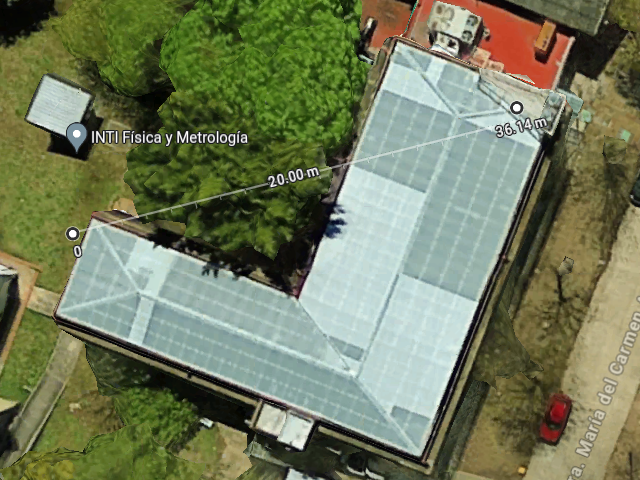
\includegraphics[width=0.6\textwidth]{./figuras/antenapos2.png}
        \caption{Posición de la antena SIM respecto de la posición de la antena del receptro GTR}
        \label{fig:antenapos2}
    \end{center}
\end{figure}

Analizo los primero resultados de medición. En la figura \ref{fig:medicionesMJD60364} se muestra en negro los valores del GTR. En varios colores, los satélites del \polar.


\begin{figure}[ht]
    \begin{center}
        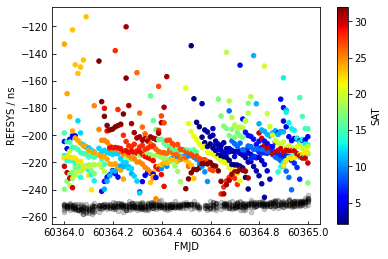
\includegraphics[width=0.6\textwidth]{./figuras/medicionesMJD60364.png}
        \caption{Primera medición con el \polar. Tomado a partir de los CGGTTS}
        \label{fig:medicionesMJD60364}
    \end{center}
\end{figure}

La media del GTR da \SI{-251.6}{\nano\second}. La del \polar  da \SI{-213.4}{\nano\second}. La diferencia es \SI{38.2}{\nano\second}. Esto correspondería al INT DELAY del \polar.


\section{28/02/2024. Análisis de datos RINEX}

Como los datos de L3 de la figura \ref{fig:medicionesMJD60364} son muy ruidosos, intento obtener por separado las componentes C1, P1, P2 a partir de los RINEX de los receptores GTR y \polar. Pruebo varios softwares. Con el que más o menos llego a algo es con el \textit{dclrinex} del BIPM, que es el que fue preparado para realziar estas mediciones. Bajo la última versión de esta página:  \href{https://webtai.bipm.org/ftp/pub/tai/publication/gnss-calibration/doc-soft/dclrinex.sh_20160322}{link dclrinex}. Viene un código Fortran y un script Bash. Intento que corra el .f. Los archivos \textit{de observación} tienen que tener el nombre en el formato SIMr0560.24O y inti0560.24O, como ejemplo para el día 56 del año 2024. Al de navegación para el mismo día hay que llamarlo \textit{BRDC00IGS\_R\_20240560000\_01D\_MN.rnx} (en el código latex, las contrabarras son para el guión bajo)

\section{29/02/2024. Análisis de datos RINEX}
Hoy sigo intentando que corra el código \textit{dclrinex.f}. El ejecutable termina compilando pero concluye con un error de división por cero para la constelación Beidu (no incluida en los datos). Pruebo con \textit{dclrinex.sh}. Tengo que instalar GMT (Generic Map tools): sudo apt-get install gmt gmt-dcw gmt-gshhg. 
Ojo que estuve modificando el script dclrinex.sh por dos cosas: Una porque llamaba a un directorio local de la computadora donde fue escrito, y otra porque la versión actual del soft gmt cambió, y lo que antes era un comando, ahora es parte de el argumento. Por ejemplo, gmt psxy.

\section{01/03/2024. Análisis de datos usando R2CGGTTS}
Con el código de ayer no hubo caso. Bijunath me recomendó subir los RINEX a la página del NRCan, pero eso sólo me genera las coordenadas cartesianas. Vuelvo a intentar con R2CGGTTS. Es el software que está en el FTP del BIPM. Está escrito en Fortran 77. Logro generar algunos CGGTTS. Comparo los CGGTTS generados por el GTR internamente y otros CGGTTS generado por este código. Hay una diferencia de 60 ns. Pero tengo que estudiarlo más.
Para que corra, tengo que utilizar el comando \textit{gfortran $-$std$=$legacy R2CGGTTSV8$\_$31.f} .


La versión $\_31$ es una modificación mía para que no genere archivos vacios de Beidu, GLONASS y GALILEO. Simplemente comenté unas líneas.

\section{07/03/2024. Análisis de datos usando R2CGGTTS}

Continué analizando los datos con el soft R2CGGTTS. 
De lo que leo, los RINEX que genera el GTR ya tienen alguna corrección incluida, pero encuentro cuál. Probé restando los delays de calibración y el REFDELAY, pero no alcanza para superponer las curvas.


\begin{figure}[ht]
    \begin{center}
        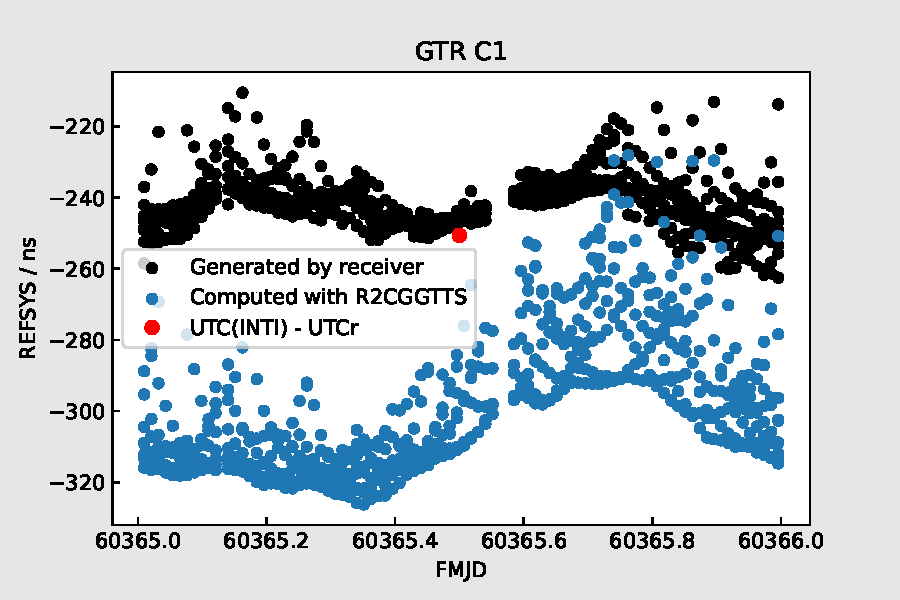
\includegraphics[width=0.45\textwidth]{./figuras/GTR-C1}
        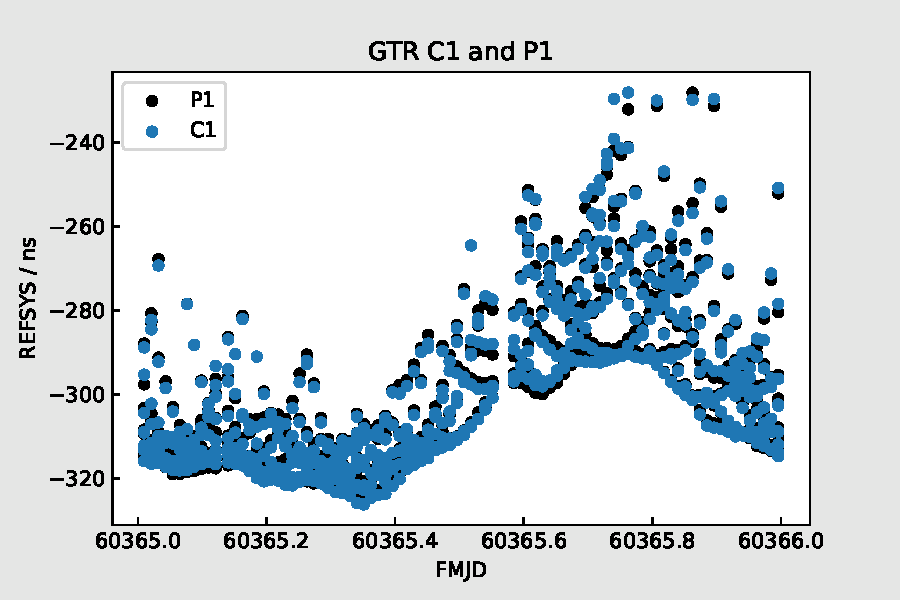
\includegraphics[width=0.45\textwidth]{./figuras/GTR-C1P1}
        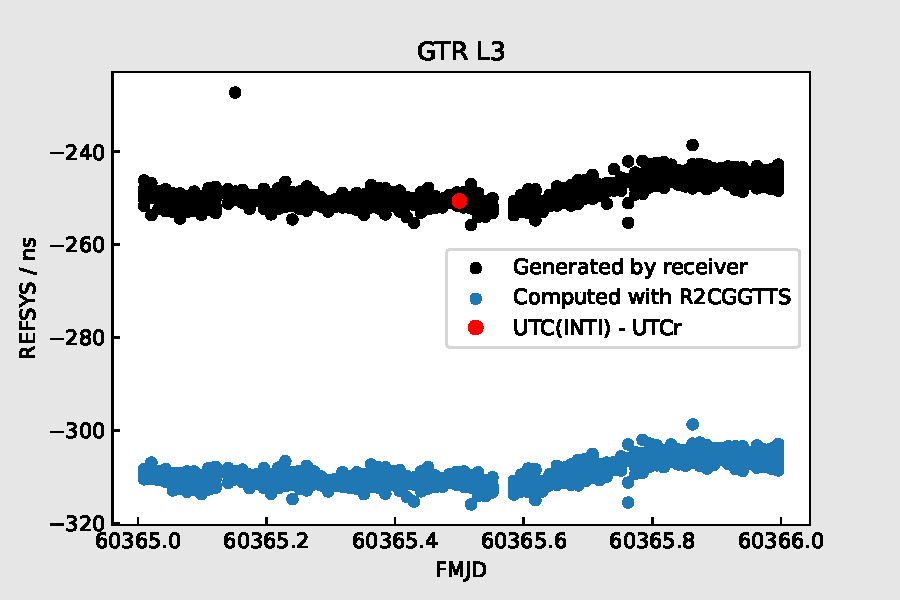
\includegraphics[width=0.45\textwidth]{./figuras/GTR-L3P}
        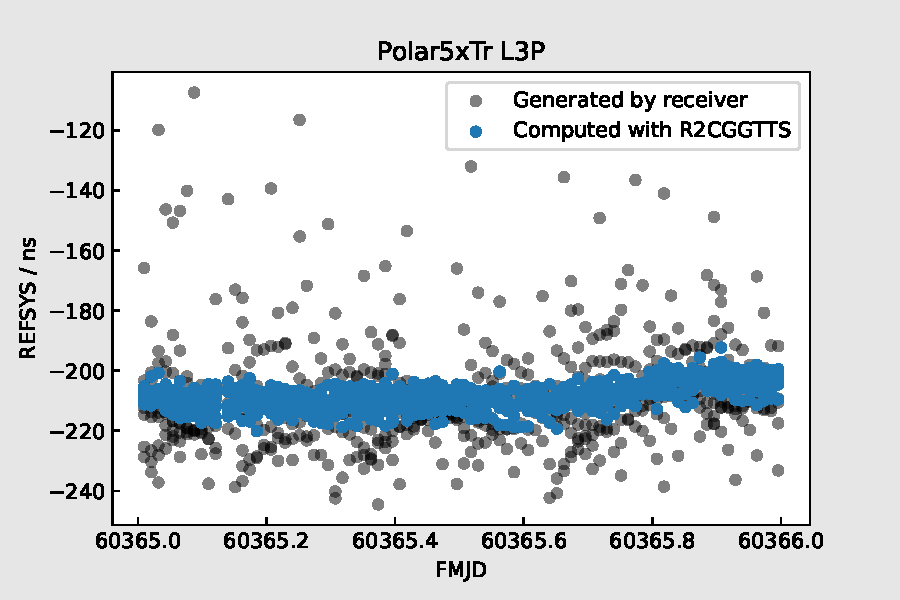
\includegraphics[width=0.45\textwidth]{./figuras/Polar5xTr-L3P}
        \caption{Calculos de diferencias de tiempo con el software R2CGGTTS}
        \label{fig:Obtencion de archivos CGGTTS a partir re RINEX}
    \end{center}
\end{figure}

\section{11/03/2024. Análisis de datos}
Continúo tratando de analizar los datos. Ahora vuelvo a intentar con el \textit{dclrinex}. Algo que es importante es pasar los scripts \textit{dclrinex.sh} y \textit{dclrinexplot.sh}  por el programa \textit{dos2unix} para compatibilizar con linux.

Lo que se muestra en la figura \ref{fig:capturaDLCRINEX} es la diferncia entre las señales del \polar y del GTR para las mediciones del 22/2/24.

\begin{figure}[ht]
    \begin{center}
        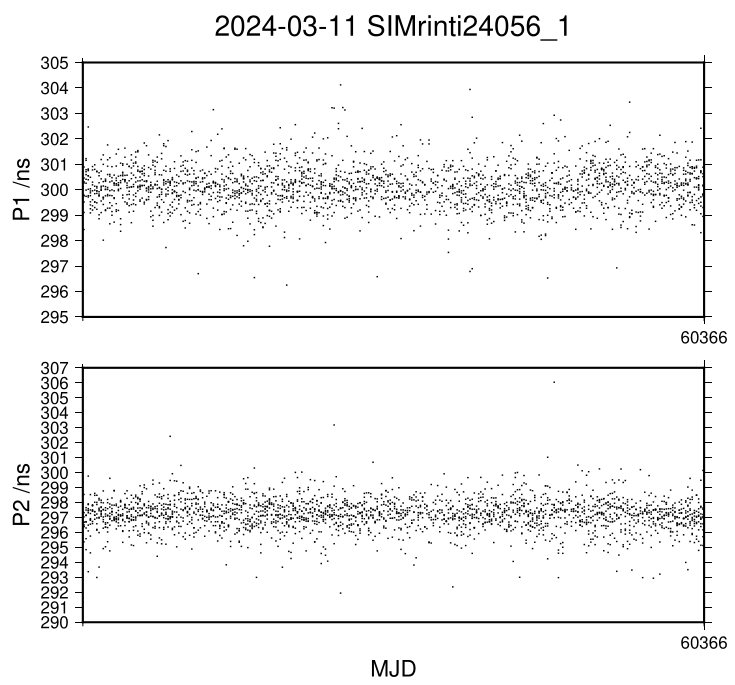
\includegraphics[width=0.6\textwidth]{./figuras/capturaDLCRINEX.png}
        \caption{Salida del soft DLCRINEX}
        \label{fig:capturaDLCRINEX}
    \end{center}
\end{figure}


\section{12/03/2024. Comienzo nueva medición con el \polar}
Comienzo una nueva medición. Continuo analizando los datos. Bajo los archivos de navegación de \url{https://cddis.nasa.gov/archive/gnss/data/daily/}

\section{14/03/2024. Primeros resultados con el soft DCLRINEX.}

Copio y pego el mail que les envié con los resultados:

Here a new update with the progress on the SIM receiver.
I switched the software DLCRINEX, which is the one that Bijunath used in the calibrations for Argentina. I had to make a few modifications, since the code was intended to be used under Windows environment. Also, some plotting modules (GMT, Generic Mapping Tools) have updated versions that are no longer compatible with the DCLRINEX code.
I have been able to extract C1, P1 and P2 differences:

If you had seen these figures before,  you may notice that the TimeDeviation plots are absent. This is due to the compatibility issues with the plotting tool that I mentioned before. However, the values are generated and stored. I plotted them and computed the stability with allantools in python. (See attached).

\begin{figure}[ht]
    \begin{center}
        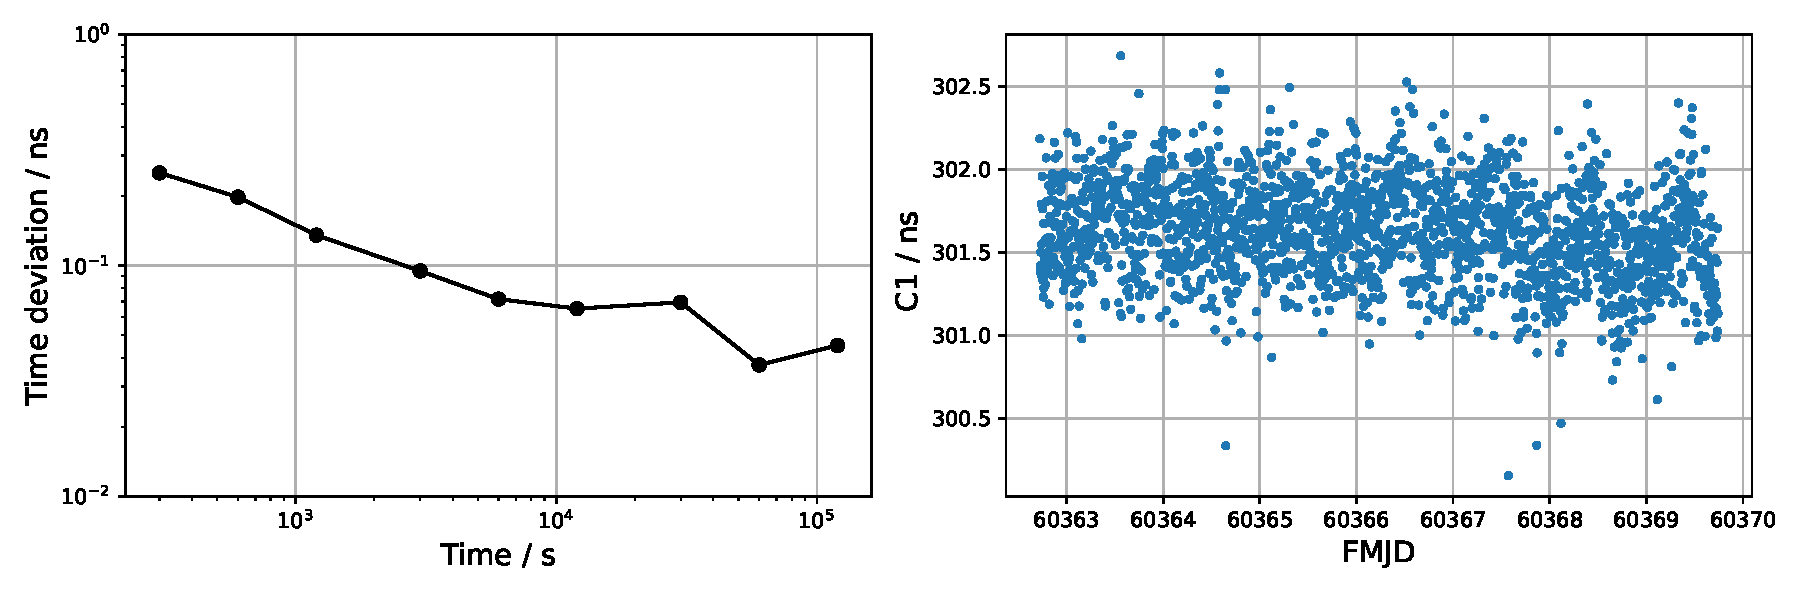
\includegraphics[width=0.8\textwidth]{./figuras/C1.pdf}
        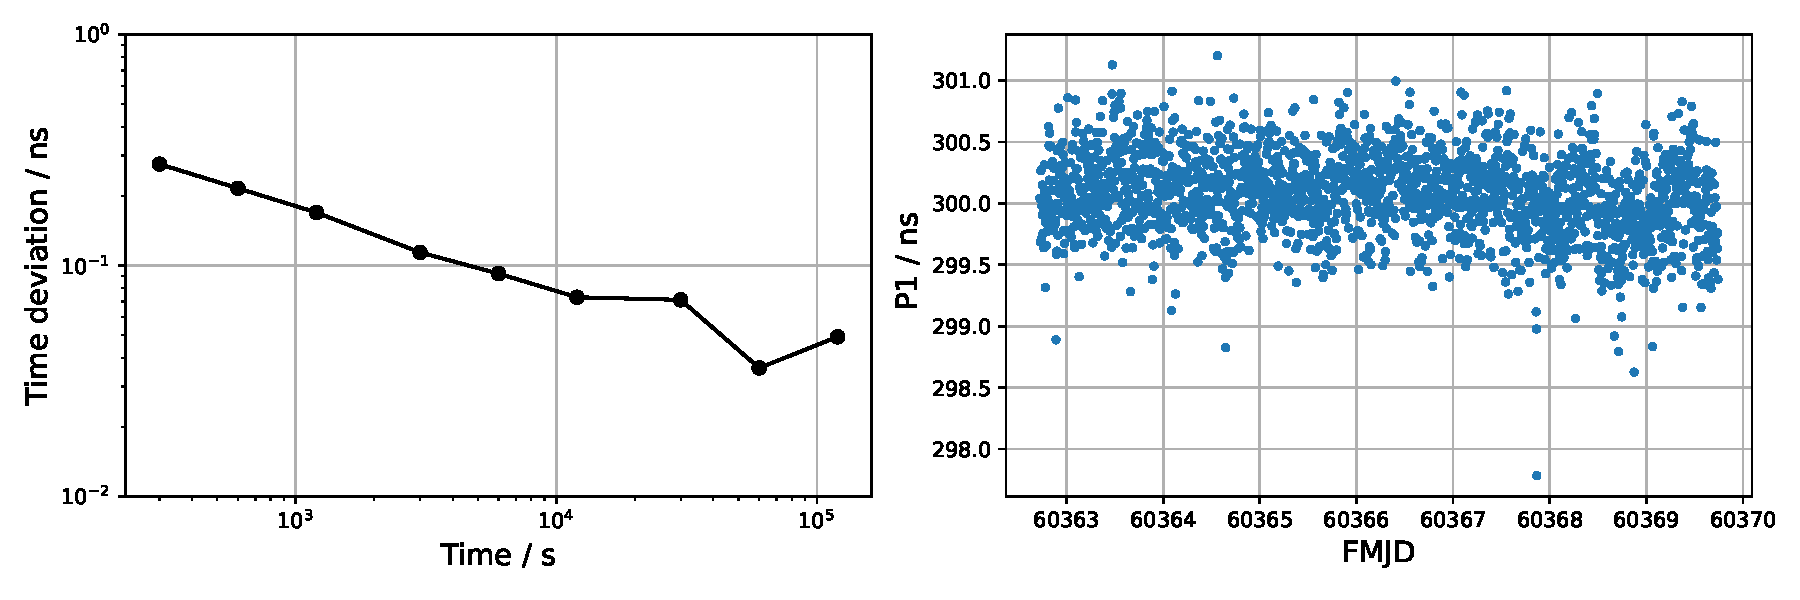
\includegraphics[width=0.8\textwidth]{./figuras/P1.pdf}
        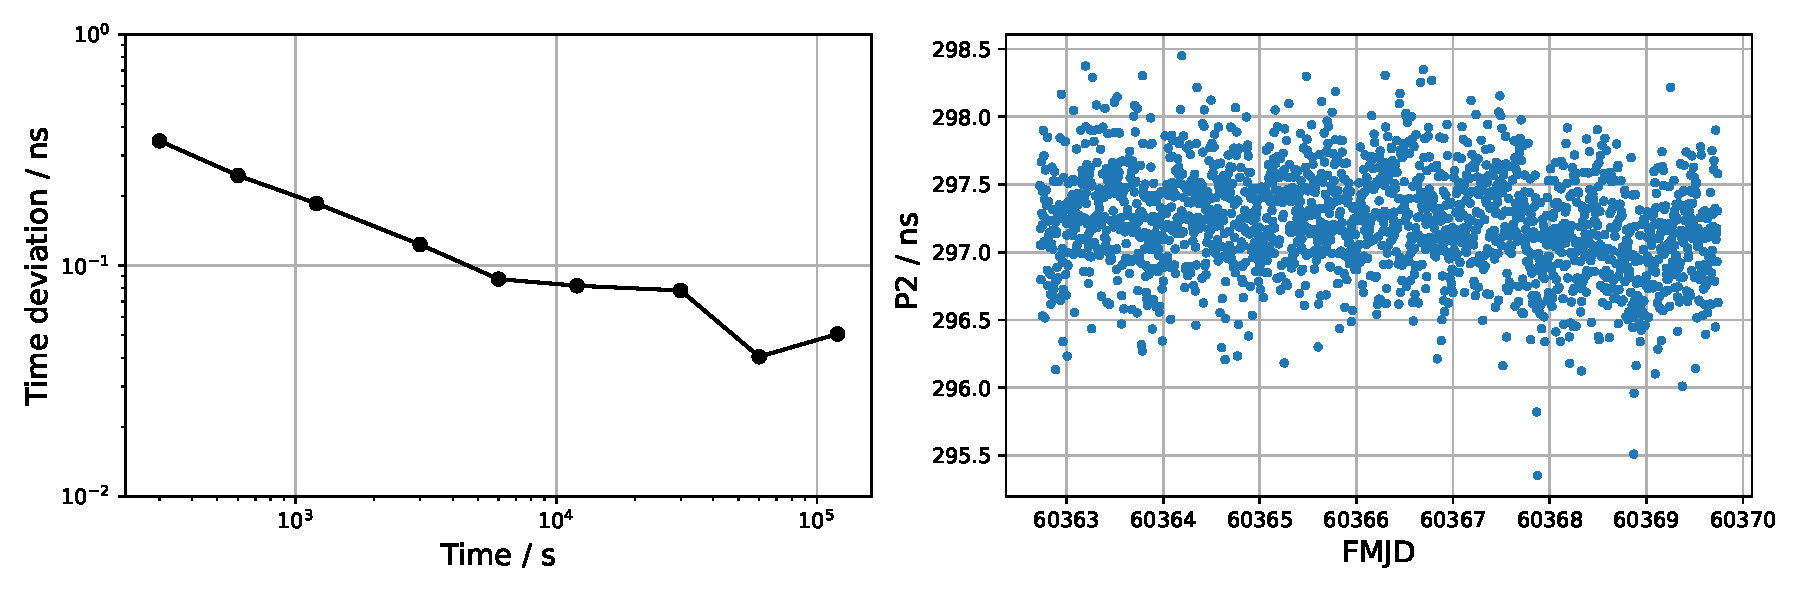
\includegraphics[width=0.8\textwidth]{./figuras/P2.pdf}
    \end{center}
\end{figure}



With these results, I computed the Internal delay of the travelling receiver. The results are: 

INTdlyC1: 33.6 ns, 

INTdlyP1: 32.1 ns, 

INTdlyP2: 29.2 ns. 

Later, I compared my results with others in the page of the BIPM of the same receiver model and, preferably,  the same antenna: (Figura \ref{fig:comparaciondelays})



\begin{figure}[ht]
    \begin{center}
        \includegraphics[width=0.6\textwidth]{./figuras/comparacionesBIPM.png}
        \caption{Comparación con otras calibraciones de receptores \polar y antenas NOVALTEL750.}
        \label{fig:comparaciondelays}
    \end{center}
\end{figure}

\section{15/03/2024. Medición de base de tiempo de contador \BNC. Comienzo de informe}

Hago una medición para ver cómo sigue el PLL del contador a los \SI{10}{\mega\hertz} de referencia externa. Hice un programa en Labview en la computadora que se usa para las calibraciones. Figura \ref{fig:BNC10MHz}

\begin{figure}[ht]
    \begin{center}
        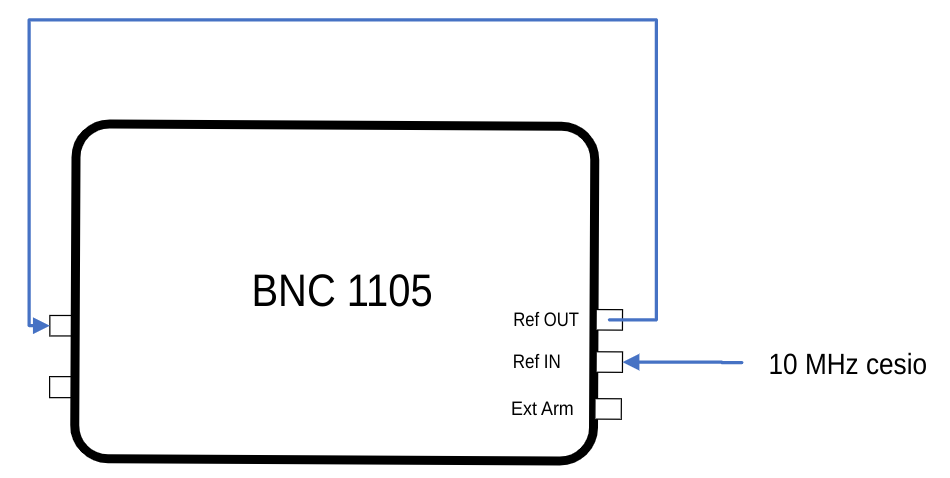
\includegraphics[width=0.5\textwidth]{./figuras/esquemaBNC.png}
        \caption{Esquema para medición de lazo PLL de contador \BNC}
        \label{fig:BNC10MHz}
    \end{center}
\end{figure}

\newpage
\section{18/03/2024. Medición de base de tiempo de contador \BNC. Comienzo de informe}

Analizo los datos de la estabilidad del contador \BNC que empecé a medir el 15 de marzo. En la figura \ref{fig:BNC10MHz_allan} se muestran los valores medidos y el desvío de allan con overlap. Es de notar que hay un offset de \SI{-2e-12}{} en la frecuencia. Con respecto al desvío de allan, se vé que posee una dependencia $t^{-1/2}$, correspondiente a un ruido random walk frequency modulation. Si se considera que la resolución del contador para 10 MHz es de \SI{0.5e-12}{}, se puede decir que se alcanza ese valor de desvío de Allan en aproximadamente 10 segundos de promediación. 

Sigo trabajando en el informe.

\begin{figure}[ht]
    \begin{center}
        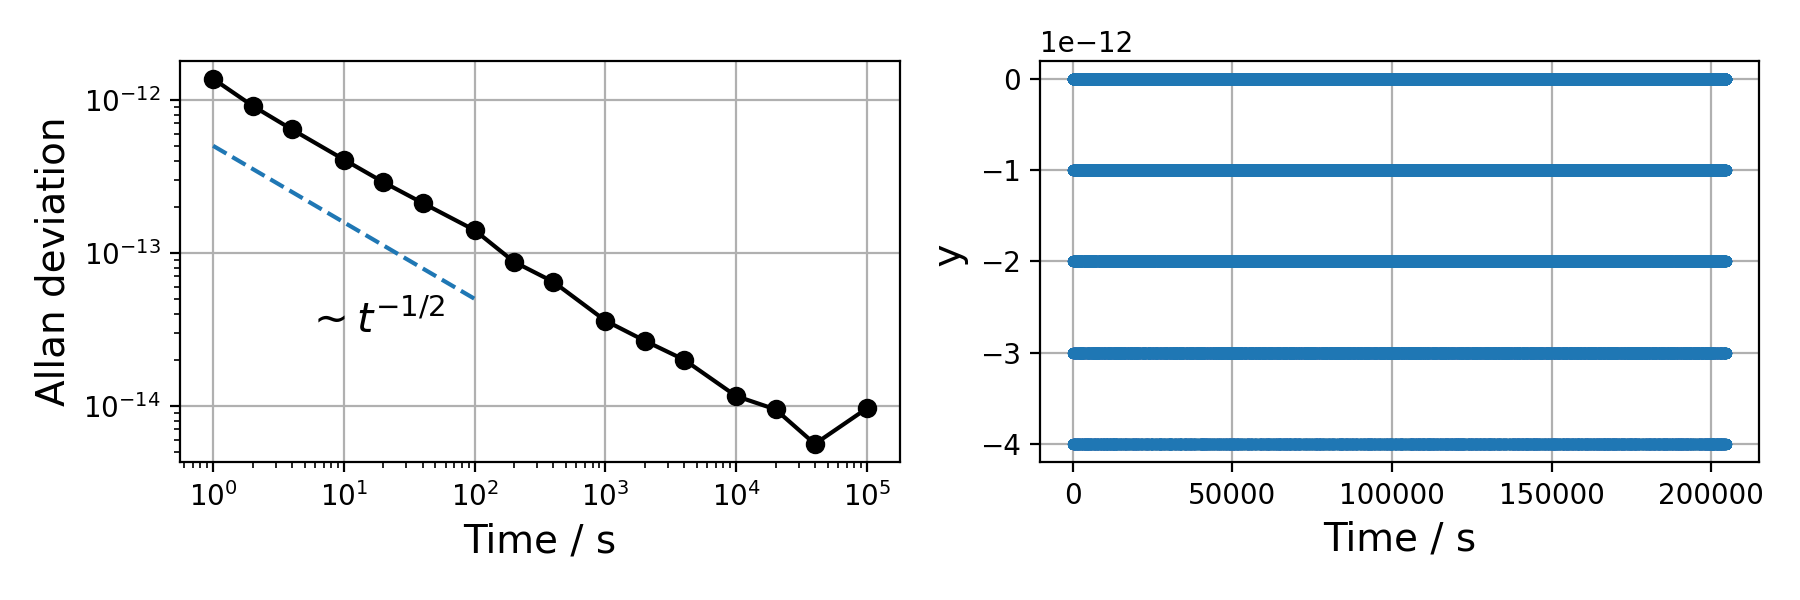
\includegraphics[width=0.8\textwidth]{./figuras/BNC10MHz_oadev.png}
        \caption{Resultados de la medición de 10 MHz del 15 de marzo}
        \label{fig:BNC10MHz_allan}
    \end{center}
\end{figure}

\section{19/03/2024. Continuo informe. Reestablezco receptor NIST-TAI1, soft para medicion de delay.}

Vuelvo a poner en funcionamiento el receptor NIST-TAI1. Mi intención es ver si puedo lograr una medición con poco ruido, para me permita comparar la calibración original del receptor con una nueva que haga contra el GTR. Continúo con el informe. Me paso a al TeXMaker, porque había problemas con la conexión o con el Overleaf. Empiezo a hacer un soft para medir el delay de la antena por varios días.

\section{22/03/2024. Continuo informe, analizo incertidumbres. Receptor NIST-TAI1}
Continuo con el informe. Termino de escribir el esqueleto, faltaría refinar los números. No termino de comprender cómo se calculan las incertidumbres. Estoy tratando de re-calcular los valores del informe de Biju, pero no me da. El problema viene con la sumatoria de las incertidumbres tipo B. Empiezo a ver por qué dejamos de usar el NIST-TAI1.

\section{25/03/2024. Final mediciones GNSS marzo. Mido $X_0$. Comienzo  medición long term cable antena}

Termino mediciones GNSS que comencé el 12/3. Mido el $X_0$ del \polar con los contadores BNC y Agilent. Me dá: $X_0 (Agilent) = 54.96$ $X_0 (BNC) = 54.82$. No es tanta la diferencia entre contadores, 0.1 ns. Sí hay diferencia con el valor medido el 19/2: 55.2 ns. Los desvíos estándar de las mediciones estaban en el orden de \SI{e-11}{\second}.

\section{03/04/2024. Final medición long term cable antena}
En los dias anteriores, estuve tratando de ver cuál era el problema del receptor NIST-TAI1. En principio había un conflicto con la hora. Le cambié la pila botón interna. Eso no solucionó nada. El tema es que cuando se larga el programa de medición toma la fecha GPS que recibe y la asigna al clock de la PC. Como demora en enganchar, le asigna una hora del 2004. Como workaround, generé un usuario sin permisos de cambiar la hora y desde ahí corrí el programa de medición. Corrió bien, pero durante el fin de semana de pascua, se reinición varias veces el receptor. Sigo viendo qué puede ser.

\begin{figure}[ht]
    \begin{center}
        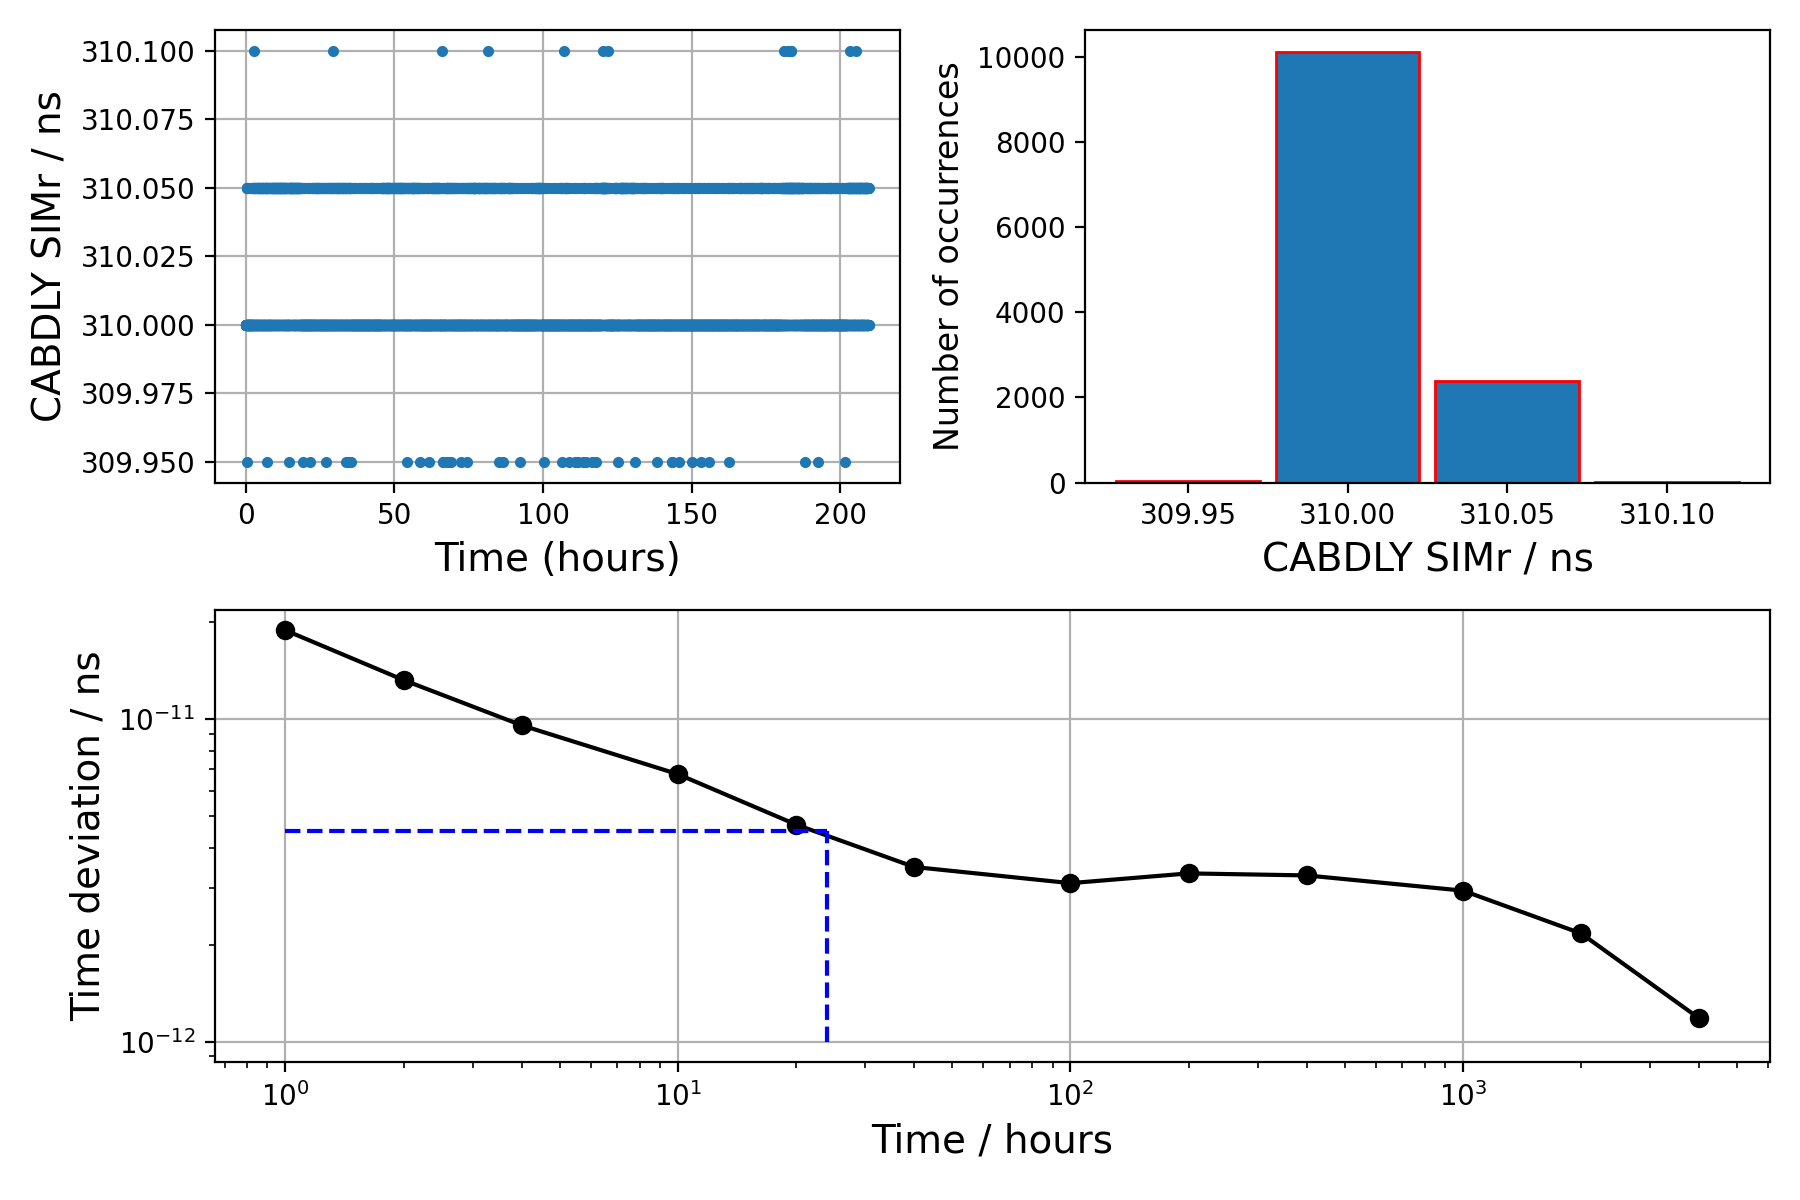
\includegraphics[width=0.8\textwidth]{./figuras/antenadelaySIMr.png}
        \caption{Medición durante 8 días del CABDLY del receptor SIMr, con el cable montado y utilizando la técnica de reflexión. Ver análisis de resultados del 4/4/2024 }
        \label{fig:antenadelaySIMr}
    \end{center}
\end{figure}

\section{4/04/2024. Análisis medición long term cable antena (ver ayer)}
La figura \ref{fig:antenadelaySIMr} dá un resultado de medición de $\boxed{\SI{310.0}{\nano\second}}$. Eso corresponde a tomar las mediciones crudas, dividirla por dos, restarle el offset ó tara de \SI{36.4}{\nano\second} y tomar la mediana.
Este valor es distinto del resultado del 8/2/2024. (La vez pasada dio $635.2/2 = 317.6$ ns ). Hay una diferencia notable, pero de todos modos, se puede ver que la la estabilidad del cable por estar expuesto a la intemperie no es un problema. La limitación de la medición está dada por la resolución del contador. En la figura \ref{fig:antenadelaySIMr} se muestra el time deviation de la medición. Las lineas punteadas corresponden a la estabilidad a $\tau = 24$ horas. Corresponde a un valor de \SI{4.5e-12}{\second}. Este valor está bien por debajo de la resolución del contador, por lo que resulta desperciable.
CLARAMENTE hay que repetir la medición. Principalmente, visualizar la señal con un osciloscopio. 
\textbf{Nota del 18/04/24: Noté que el programa corrió con una impedancia de 1M en el canal 1. Hay que repetir esta medición para obtener un valor absoluto representativo. Pero para la estimación de la estabilidad, la medición sirve.}

\section{5/04/2024. Análisis medición GNSS marzo del 2024}
Analizo los datos de las mediciones que largué el 12/03/2024. Los gráficos se ven muy parecidos. Volví a usar \textit{dclrinex}. El comando fue: \texttt{\$ dclrinex SIMr inti 24072 14 }

Resumo los datos en la tabla 


\begin{table}[h]
    \centering
    \begin{tabular}{lcc}
         &  February 2024 & March 2024 \\
         \hline
    INTdlyC1     & \SI{33.62}{\nano\second}& \SI{33.72}{\nano\second}\\
    INTdlyP1     & \SI{32.07}{\nano\second}& \SI{32.12}{\nano\second}\\
    INTdlyP2     & \SI{29.20}{\nano\second}& \SI{29.35}{\nano\second}\\
    \end{tabular}
    \caption{Comparacion de resultados de calibracion del receptor en dos campañas: febrero y marzo de 2024}
    \label{tab:febrero-marzo}
\end{table}

\section{09/04/2024. Medición de cable de antena montado}

Vuelvo a repetir la medición tomando un promedio de 100 lecturas con el BNC del delay de la antena (Repito la medición del 4/4). Ahora me da: $692.62/2-36.17 = \SI{310.14}{\nano\second}$. Es decir, de 5 días hasta hoy, la diferencia con la tecnica de reflexion y el cable montado es de \SI{0.14}{\nano\second}

\section{12/04/2024. Medición de cable de antena montado (repito)}
Dejé la medición andando desde el 9/4/2024. Los valores son los mismos desde entonces.

\section{17/04/2024. Tercera medición GNSS}
Comienzo por medir el $X_0$. Me dá $X_0 = \SI{95.42}{\nano\second} - \SI{41.66}{\nano\second} = \SI{53.76}{\nano\second}$. Hay una diferencia con respecto de los 55.2 nano que nos dio el 19/02/2024. Según el manual de Biju, esto puede variar, pero no entiendo bien por qué.\\

Intento ver cómo se comporta con el valor de $X_0$ compensado internamente. Me arroja una lectura muy variable. Vuelvo a deshabilitar la opción de compensación interna.

Ahora obtengo dá $X_0 = \SI{96.09}{\nano\second} - \SI{41.66}{\nano\second} = \SI{54.43}{\nano\second}$. La tara no la repetí.

\section{30/04/2024. Análisis de tercera medición GNSS (falló)}

No pude procesar los datos de abril 2024. La salida del dclrinex me tira archivos vacios. Estimo que se debe a que las mediciones se realizaron cada un minuto, y el soft asume que son cada 30 segundos. Vuelvo a largar una medición (que será más corta), ahora con RINEX a 30 segundos. 

\textbf{ES IMPRESCINDIBLE QUE LOS RINEX A COMPARAR TENGAN EL MISMO INTERVALO DE TIEMPO (30 SEGUNDOS)}


Lo que sí pude hacer es levantar las mediciones de REFDLY durante los 10 días que dejé midiendo. Esto es lo que da:


\begin{figure}[ht]
    \begin{center}
    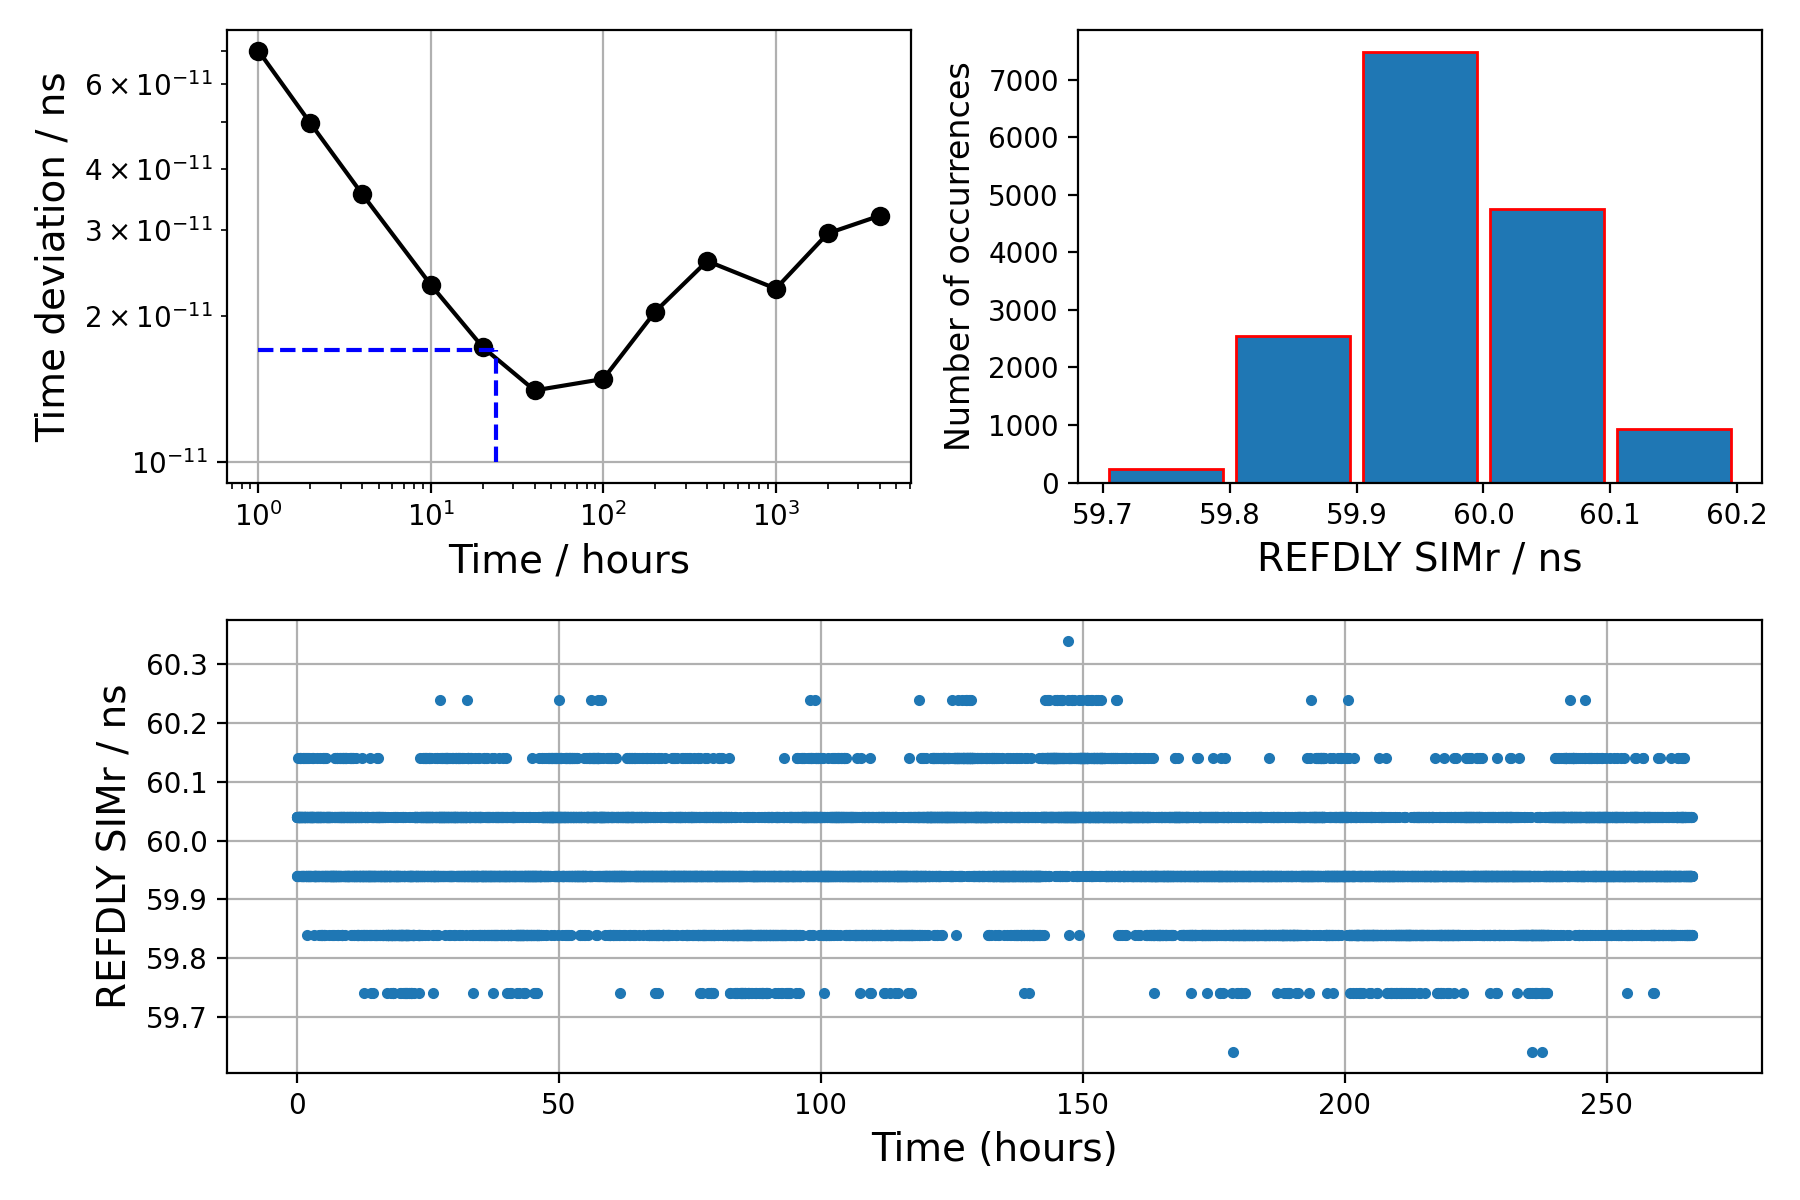
\includegraphics[width=0.8\textwidth]{./figuras/REFDLY_SIMr.png}
        \caption{Resultados de la medición de REFDLY durante abril 2024}
        \label{fig:REFDLY_longterm}
    \end{center}
\end{figure}

A un día de medición, el Time deviation me da \SI{0.02}{\nano\second}.


Hacemos una llamada con Víctor y Mauricio de AGGO. Quedamos en que arreglamos con Alfredo para llevar el receptor SIMr a AGGO.

Largo otra medición GNSS. 

\section{2/05/2024}
Para la medición que largué el 30/4 me olvidé de medir el REFDLY. Hoy me dá $X_0= 96 - 41.6= \SI{54.4}{\nano\second}$. Hago un análisis de los resultados del 1/5. Uso sólo un dia, pero es para verificar que esté bien configurado el receptor. Me da: $RAWDIFF(C1) = -302.1$, $RAWDIFF(P1) = -300.4$, $RAWDIFF(P2) = -297.7$. Esto es aproximadamente $+\SI{0.4}{\nano\second}$ que en la medición de marzo. (Ver el Excel en la carpeta)  

\section{15/05/2024}
Detengo la medición. El $X_0$ me da $X_0= 96.17 -41.6 = \SI{54.57}{\nano\second}$. Teniendo en cuenta el delay del cable, me queda $REFDLY_{Polar}= \SI{60.07}{\nano\second}$.




\newpage
\printbibliography[title= Referencias, heading=bibintoc]


\end{document}


